%%%%%%%%%%%%%%%%%%%%%%%%%%%%%%%%%%%%%%%%%%
% Mathematics Final Year Research Projects
% LaTeX Template
% Version 1.0 (31/01/24)
%
% This template has been adapted from: https://www.overleaf.com/latex/templates/imperial-college-report-template/wncnzptkhnbc
% Students should feel free to adapt this template to their needs.
%%%%%%%%%%%%%%%%%%%%%%%%%%%%%%%%%%%%%%%%%%
%----------------------------------------------------------------------------------------
% PACKAGES AND OTHER DOCUMENT CONFIGURATIONS
%----------------------------------------------------------------------------------------

% IMPORTANT NOTE: This version of the document is NOT the one I'm submitting. This is a significantly longer version that contains several important details that can later be added to the blueprint. The text here, particularly in Chapter 4, is meant to mimic the arguments that we have and will formalise.

\documentclass[a4paper,11pt, twoside]{report}
\usepackage[T1]{fontenc}
\usepackage[utf8]{inputenc}

%% Language and font encodings
\usepackage[english]{babel}
\usepackage[utf8]{inputenc}
\usepackage[T1]{fontenc}

%% Imperial Recommended Packages
\usepackage{afterpage}

% Lean colour configurations
\usepackage{color}
\definecolor{keywordcolor}{rgb}{0.7, 0.1, 0.1}   % red
\definecolor{tacticcolor}{rgb}{0.0, 0.1, 0.6}    % blue
\definecolor{commentcolor}{rgb}{0.4, 0.4, 0.4}   % grey
\definecolor{symbolcolor}{rgb}{0.0, 0.1, 0.6}    % blue
\definecolor{sortcolor}{rgb}{0.1, 0.5, 0.1}      % green
\definecolor{attributecolor}{rgb}{0.7, 0.1, 0.1} % red
\definecolor{backcolour}{rgb}{0.95,0.95,0.92}

% Listings (for displaying code):
\usepackage{listings}
\def\lstlanguagefiles{TeX_Setup/lstlean.tex}
\lstset{
    % frame = single, 
    % framexleftmargin=15pt,
    language = lean,
    numbers = left,
    backgroundcolor=\color{backcolour},
    inputencoding=ansinew,
    % extendchars=\true
}

% ----------- Algorithm2e setup
\usepackage[ruled,vlined]{algorithm2e}
\makeatletter
\renewcommand{\SetKwInOut}[2]{%
  \sbox\algocf@inoutbox{\KwSty{#2}\algocf@typo:}%
  \expandafter\ifx\csname InOutSizeDefined\endcsname\relax% if first time used
    \newcommand\InOutSizeDefined{}\setlength{\inoutsize}{\wd\algocf@inoutbox}%
    \sbox\algocf@inoutbox{\parbox[t]{\inoutsize}{\KwSty{#2}\algocf@typo:\hfill}~}\setlength{\inoutindent}{\wd\algocf@inoutbox}%
  \else% else keep the larger dimension
    \ifdim\wd\algocf@inoutbox>\inoutsize%
    \setlength{\inoutsize}{\wd\algocf@inoutbox}%
    \sbox\algocf@inoutbox{\parbox[t]{\inoutsize}{\KwSty{#2}\algocf@typo:\hfill}~}\setlength{\inoutindent}{\wd\algocf@inoutbox}%
    \fi%
  \fi% the dimension of the box is now defined.
  \algocf@newcommand{#1}[1]{%
    \ifthenelse{\boolean{algocf@inoutnumbered}}{\relax}{\everypar={\relax}}%
%     {\let\\\algocf@newinout\hangindent=\wd\algocf@inoutbox\hangafter=1\parbox[t]{\inoutsize}{\KwSty{#2}\algocf@typo\hfill:}~##1\par}%
    {\let\\\algocf@newinout\hangindent=\inoutindent\hangafter=1\parbox[t]{\inoutsize}{\KwSty{#2}\algocf@typo:\hfill}~##1\par}%
    \algocf@linesnumbered% reset the numbering of the lines
  }}%
\makeatother
% --------- end algorithm2e setup

\usepackage{bm}
\usepackage[normalem]{ulem}

\usepackage[colorinlistoftodos]{todonotes}

% I have all of their other recommended packages somewhere on here.

\usepackage[most]{tcolorbox}
\usepackage{authblk}  % Lets you add an \affil{} to your title, stating your affiliation {eg. Sigma Mathematics Society}
\usepackage{ragged2e}
\usepackage{csquotes}
\usepackage{pdfpages}



\usepackage{xfrac}
\usepackage{cancel}

\usepackage[inline]{enumitem}

%\usepackage{tgpagella}

\usepackage{blindtext}
\usepackage{lipsum}
\usepackage{verbatim}
\usepackage{hyperref}
\hypersetup{
    citebordercolor = 1 1 1,
    linkbordercolor = 1 1 1,
    filebordercolor = 1 1 1,
    menubordercolor = 1 1 1,
    urlbordercolor = 1 1 1,
    colorlinks  =   true,
    linkcolor   =   blue,
    citecolor   =   magenta,
    urlcolor    =   blue
}

% This project uses natbib instead. See end of format file.
% \usepackage{biblatex} % Modify citation format using [style=yourstyle] parameter--eg \usepackage[style=mla-new]{biblatex}
% \bibliography{TeX_Setup/References.bib}
% \addbibresource{TeX_Setup/References.bib}

\usepackage{cancel}
\usepackage{amssymb}
\usepackage{amsmath}
% \usepackage{amsthm}  % In `environments.tex`
%\usepackage{MnSymbol}
\usepackage{mathrsfs}
\usepackage{mathtools}
% \usepackage{mathabx}
\usepackage{mathdots}
\usepackage{yhmath}

\usepackage{array}
\usepackage{booktabs}
\usepackage{longtable}

\usepackage{graphicx}
\newcommand\sbullet[1][.5]{\mathbin{\vcenter{\hbox{\scalebox{#1}{$\bullet$}}}}}  % Bullet of customisable size
\usepackage{wrapfig}
% Imperial-recommended `caption` setup
\usepackage{caption}
\captionsetup[figure]{labelfont={bf}, name={Figure}, justification=centering}
\captionsetup[table]{labelfont={bf}, name={Table}}
\usepackage{subcaption}
\usepackage{tikz}
\usepackage{float}

% Tikz
\usepackage{tikz-cd}
\usepackage{tikz-3dplot}
\usetikzlibrary{positioning}
\usetikzlibrary{cd}
\usetikzlibrary{shapes.geometric}
\usepackage{pgfplots}
\usepackage{mathrsfs}
\usetikzlibrary{arrows}
\usepackage{qtree}

%% Sets page size and margins
\usepackage[a4paper,top=1in,bottom=1in,left=1in,right=1in,marginparwidth=1.75cm]{geometry}

% Font

% \usepackage{sansmathfonts}
% % \usepackage{mathrsfs}
% \usepackage[T1]{fontenc}
% \renewcommand*\familydefault{\sfdefault}

\renewcommand*{\rmdefault}{bch}
\renewcommand*{\ttdefault}{lmtt}

% Structure and Numbering

\usepackage{fancyhdr}
\usepackage{lastpage}

\pagestyle{fancy}
\fancyhf{}

\rhead{{Page \thepage}}%\hspace{1pt} of \pageref{LastPage}}}
\lhead{\textit\slshape\nouppercase{\leftmark}}

\numberwithin{equation}{section}

% Lists

\setlist[description]{font=\normalfont}
\setlist[enumerate]{font=\normalfont}

% Spacing and indentation

% Not sure if 1.5-spacing is permitted. I'll leave it commented out for now.
% \usepackage{setspace}
% \renewcommand{\baselinestretch}{1.5}

\usepackage[skip=11pt, indent=0pt]{parskip}
% Here's what Imperial's recommended setup is:
% \setlength{\parskip}{0.5em}
% \usepackage{indentfirst}  % Uncomment if using above

\allowdisplaybreaks  % Allows align environments to continue for several pages

% Colours

\usepackage{xcolor}
\definecolor{darkblue}{rgb}{0.0, 0.0, 0.55}
\definecolor{pink}{rgb}{0.858, 0.188, 0.478}
\definecolor{brown}{rgb}{0.8, 0.4, 0.0}

% Bibliography
\usepackage[numbers, comma, square, sort&compress]{natbib}
\bibliographystyle{References/abbrvunsrtnat.bst}
% \bibliographystyle{unsrtnat}

\usepackage{amsthm}
\usepackage{cleveref}

\newtheorem*{theorem*}{Theorem}
\newtheorem{theorem}{Theorem}[section]
\newtheorem{corollary}[theorem]{Corollary}%[theorem]
\newtheorem{lemma}[theorem]{Lemma}
\newtheorem{claim}[theorem]{Claim}
\newtheorem{conjecture}[theorem]{Conjecture}
% \newtheorem{algorithm}[theorem]{Algorithm}  % Defined in algorithm2e
\newtheorem{proposition}[theorem]{Proposition}

\newtheorem{problem}[theorem]{Problem}
\newenvironment{boxproblem}{
    \begin{tcolorbox}[colback=black!25!orange,colframe=black!50!orange, coltext=white, breakable, enhanced]\begin{problem}
}{
    \end{problem}\end{tcolorbox}
}

\newenvironment{boxtheorem}{
    \begin{tcolorbox}[colback=yellow!15!white,colframe=orange, breakable, enhanced]\begin{theorem}
}{
    \end{theorem}\end{tcolorbox}
}
\newenvironment{boxproposition}{
    \begin{tcolorbox}[colback=yellow!15!white,colframe=orange, breakable, enhanced]\begin{proposition}
}{
    \end{proposition}\end{tcolorbox}
}
\newenvironment{boxlemma}{
    \begin{tcolorbox}[colback=yellow!15!white,colframe=orange, breakable, enhanced]\begin{lemma}
}{
    \end{lemma}\end{tcolorbox}
}
\newenvironment{boxcorollary}{
    \begin{tcolorbox}[colback=yellow!15!white,colframe=orange, breakable, enhanced]\begin{corollary}
}{
    \end{corollary}\end{tcolorbox}
}
\newenvironment{boxconjecture}{
    \begin{tcolorbox}[colback=yellow!15!white,colframe=orange, breakable, enhanced]\begin{conjecture}
}{
    \end{conjecture}\end{tcolorbox}
}


\theoremstyle{remark}
\newtheorem*{remark}{Remark}
\newtheorem*{solution}{Solution}

\theoremstyle{definition}
\newtheorem{definition}[theorem]{Definition}
\newenvironment{boxdefinition}{
    \begin{tcolorbox}[colback=cyan!10!white,colframe=cyan!70!black, breakable, enhanced]\begin{definition}
}{
    \end{definition}\end{tcolorbox}
}
\newtheorem*{convention}{Convention}
\newenvironment{boxconvention}{
    \begin{tcolorbox}[colback=magenta!3!white,colframe=magenta!70!black, breakable, enhanced]\begin{convention}
}{
    \end{convention}\end{tcolorbox}
}
\newtheorem*{notation}{Notation}
\newenvironment{boxnotation}{
    \begin{tcolorbox}[colback=magenta!3!white,colframe=magenta!70!black, breakable, enhanced]\begin{notation}
}{
    \end{notation}\end{tcolorbox}
}
\newtheorem{example}[theorem]{Example}
\newenvironment{boxexample}{
    \begin{tcolorbox}[colframe=green!30!black, breakable, enhanced, breakable, enhanced]\begin{example}
}{
    \end{example}\end{tcolorbox}
}
\newtheorem{nexample}[theorem]{Non-Example}
\newenvironment{boxnexample}{
    \begin{tcolorbox}[colframe=red!50!black, breakable, enhanced]\begin{nexample}
}{
    \end{nexample}\end{tcolorbox}
}
\newtheorem{cexample}[theorem]{Counterexample}
\newenvironment{boxcexample}{
    \begin{tcolorbox}[colframe=red!50!black, breakable, enhanced]\begin{cexample}
}{
    \end{cexample}\end{tcolorbox}
}

% \def\SMALLCOLWIDTH{1.5cm}
\newcolumntype{C}[1]{>{\centering\let\newline\\\arraybackslash\hspace{0pt}}m{#1}}

% Centering captions
% \renewcommand{\caption}[1]{\caption{\centering #1}}

\input{TeX_Setup/shortcuts.tex}

% %% Useful packages
% \usepackage{afterpage}
% \usepackage{amsmath}
% \usepackage{amsthm}
% \usepackage{amssymb}
% \usepackage{csquotes}
% \usepackage{enumitem}
% \usepackage{graphicx}
% \usepackage{lipsum}
% \usepackage{booktabs}

% % Listings (for displaying code):
% \usepackage{listings}
% \lstset{
%     frame = single, 
%     framexleftmargin=15pt
% }

% % Center figure captions:
% \usepackage{caption}
% \captionsetup[figure]{labelfont={bf},name={Figure},labelsep=quad}
% \captionsetup[table]{labelfont={bf},name={Table},labelsep=quad}


% % ----------- Algorithm2e setup
% \usepackage[ruled,vlined]{algorithm2e}
% \makeatletter
% \renewcommand{\SetKwInOut}[2]{%
%   \sbox\algocf@inoutbox{\KwSty{#2}\algocf@typo:}%
%   \expandafter\ifx\csname InOutSizeDefined\endcsname\relax% if first time used
%     \newcommand\InOutSizeDefined{}\setlength{\inoutsize}{\wd\algocf@inoutbox}%
%     \sbox\algocf@inoutbox{\parbox[t]{\inoutsize}{\KwSty{#2}\algocf@typo:\hfill}~}\setlength{\inoutindent}{\wd\algocf@inoutbox}%
%   \else% else keep the larger dimension
%     \ifdim\wd\algocf@inoutbox>\inoutsize%
%     \setlength{\inoutsize}{\wd\algocf@inoutbox}%
%     \sbox\algocf@inoutbox{\parbox[t]{\inoutsize}{\KwSty{#2}\algocf@typo:\hfill}~}\setlength{\inoutindent}{\wd\algocf@inoutbox}%
%     \fi%
%   \fi% the dimension of the box is now defined.
%   \algocf@newcommand{#1}[1]{%
%     \ifthenelse{\boolean{algocf@inoutnumbered}}{\relax}{\everypar={\relax}}%
% %     {\let\\\algocf@newinout\hangindent=\wd\algocf@inoutbox\hangafter=1\parbox[t]{\inoutsize}{\KwSty{#2}\algocf@typo\hfill:}~##1\par}%
%     {\let\\\algocf@newinout\hangindent=\inoutindent\hangafter=1\parbox[t]{\inoutsize}{\KwSty{#2}\algocf@typo:\hfill}~##1\par}%
%     \algocf@linesnumbered% reset the numbering of the lines
%   }}%
% \makeatother
% % --------- end algorithm2e setup

% % \bm allows typing bold math:
% \usepackage{bm}
% \usepackage[normalem]{ulem}

% \usepackage[colorinlistoftodos]{todonotes}
% \usepackage[colorlinks=true, allcolors=blue]{hyperref}

% \renewcommand*{\rmdefault}{bch}
% \renewcommand*{\ttdefault}{lmtt}
% \newcommand{\citationneeded}{\textcolor{red}{[citation-needed]}}

% % Add bigger skip between paragraphs, makes reading easier:
% \setlength{\parskip}{0.5em}

% % Bibliography
% \usepackage[numbers, comma, square, sort&compress]{natbib}
% \bibliographystyle{References/abbrvunsrtnat.bst}

%----------------------------------------------------------------------------------------
% END OF DOCUMENT CONFIGURATION
%----------------------------------------------------------------------------------------

%----------------------------------------------------------------------------------------
% IMPORTANT INFORMATION TO MODIFY FOR THE TITLE PAGE
%----------------------------------------------------------------------------------------
\newcommand{\reporttitle}{Viazovska's Magic Function in Dimension 8: \\ An Attempt at Formalisation} % Title of your research project
\newcommand{\reportauthor}{Sidharth Hariharan} % First Name and Last Name
\newcommand{\supervisor}{Bhavik Mehta} % First Name and Last Name of your supervisor(s)
\newcommand{\degreetype}{MSci in Mathematics} % MSci in Mathematics, BSc in Mathematics, BSc in Mathematics with Statistics, ...
%----------------------------------------------------------------------------------------

%----------------------------------------------------------------------------------------
% To compile this file, use the following sequence: 
%	latex main.tex
%	bibtex main.tex
%	latex main.tex
%	latex main.tex
%----------------------------------------------------------------------------------------

%----------------------------------------------------------------------------------------
% START OF DOCUMENT
%----------------------------------------------------------------------------------------
\begin{document}

% Title page
\begin{titlepage}

\newcommand{\HRule}{\rule{\linewidth}{0.5mm}} % Defines a new command for the horizontal lines, change thickness here

%----------------------------------------------------------------------------------------
%	LOGO SECTION
%----------------------------------------------------------------------------------------

\includegraphics[width=8cm]{Title/logo.png}\\[1cm] % Include a department/university logo - this will require the graphicx package
 
%----------------------------------------------------------------------------------------

\center % Center everything on the page

%----------------------------------------------------------------------------------------
%	HEADING SECTIONS
%----------------------------------------------------------------------------------------

% For M3R or M4R reports, comment out as appropriate
\textsc{\LARGE Imperial College London}\\[0.5cm] % Name of your university/college
\textsc{\Large Department of Mathematics}\\[1.5cm] % Name of your department
\textsc{\Large MSci Research Project}\\[0.5cm] % Name of your programme
%\textsc{\LARGE BSc Research Project}\\[1.5cm] 

%----------------------------------------------------------------------------------------
%	TITLE SECTION
%----------------------------------------------------------------------------------------
\makeatletter
\HRule \\[0.6cm]
{ \huge \bfseries \reporttitle}\\[0.6cm] % Title of your document
\HRule \\[1.5cm]
 
%----------------------------------------------------------------------------------------
%	AUTHOR SECTION
%----------------------------------------------------------------------------------------

\begin{minipage}{0.4\textwidth}
\begin{flushleft} \large
\emph{Author:}\\
\reportauthor % Your name
\end{flushleft}
\end{minipage}
~
\begin{minipage}{0.4\textwidth}
\begin{flushright} \large
\emph{Supervisor(s):} \\
\supervisor % Supervisor's name
\end{flushright}
\end{minipage}\\[2cm]
\makeatother

%----------------------------------------------------------------------------------------
%	FOOTER & DATE SECTION
%----------------------------------------------------------------------------------------
\vfill % Fill the rest of the page with whitespace
This thesis was submitted in partial fulfilment of the requirements for the \degreetype~at Imperial College London on June 9, 2025. This document is a post-submission revision that is relevant to a broader project of which the research outlined in this thesis is an important part. This version of the document is dated
\\[0.5cm]

\makeatletter
{\large \today}\\[2cm] % Date, change the \today to a set date if you want to be precise
\makeatother

\end{titlepage}

% Abstract
\thispagestyle{empty}
\begin{abstract}
    In 2022, Maryna Viazovska was awarded the Fields Medal for an outstanding achievement: solving the sphere packing problem in dimension $8$. The ingenuity of Viazovska's solution stems from her combination of techniques from the apparently unrelated theories of radial Schwartz functions and modular forms. Her proof involves constructing the so-called Magic Function, which, in this report, we will understand to be worthy of its name.

    In addition to offering an exposition of Viazovska's work, we describe important progress made in the ongoing attempt to formalise Viazovska's remarkable solution in the Lean Theorem Prover. This is a large-scale, ongoing endeavour, and we highlight the author's involvement and contributions to the effort.
\end{abstract}
 
% % Acknowledgements
% \clearpage
% \thispagestyle{empty}
\section*{Acknowledgments}

\textit{I would like to dedicate this project to my two beloved Thathas, both of whom attained Moksha during my time at Imperial. While I knew your beginnings were humble, I wish I had realised, when you were still in this world, just how much you did so that your children could have better opportunities than you. As have they, I shall ever strive to pay it forward, and completing this degree is the first step towards doing that. Not a day goes by when I do not miss you, and I will forever be grateful for all you have given me. Om Shanti.}

To my supervisor, Bhavik, I am beyond grateful for your guidance and support throughout this project. I would never have thought a chance encounter in Lausanne would lead to a working relationship that would so significantly impact my professional outlook. You have given me new standards to aspire to early on in my career, with your sharpness of mind and vastness of knowledge. Beyond a supervisor, you have been an incredible mentor and gave me great advice when I was applying to PhD positions. From the bottom of my heart, thank you.

I would further like to express my thanks to Kevin Buzzard for having not only introduced me to Lean but for never having stopped encouraging me since I attended my first Xena Project session in October 2021. I am especially grateful to you for having simultaneously hyped me up for this very high-profile project and fended off the FRO's requests to take the project public before the M4R deadline.

I would be remiss without thanking the great Maryna Viazovska herself, for whose work I have developed the profoundest appreciation over the course of this project. Even beyond that, your incredible warmth and approachability demonstrate that the greatest mathematicians are also great human beings. It has been my life's greatest honour to work with you.

I am grateful to the entire Lean community, particularly those based in London, and within that subset, those who attend Xena. I would particularly like to express my thanks to Heather Macbeth for her riveting metaprogramming sessions, one of which led to \lstinline|norm_numI|, and Edison Xie, for conversations, company, Lean brainstorming, and the occasional Michelin-star dinner.

Amma, Appa, I do not even know where I would begin. From listening to me ramble about abstract nonsense to sharing in all my joys and sadnesses, you are more than just the pillars of my world: you are my world. All I do, all I am, all I will be are because you made me so. I was blessed to be born to you.

Finally, I wish to thank everyone from my Wilkinson and maths family who has made Imperial feel like home. To my very first maths friends, Dev and Jaimin, thank you for the laughs, the vibes, and above all, for the solidarity. Without the two of you, Tarun, Krish, Arnav and Lisanne, this degree wouldn't have been nearly as fun. To the Wilkinsonians as well, from May and Amna, who have become such important figures in my life in just 8 months, to the two lights of my life, Ankita and Aarya, I am forever grateful. Before meeting you, I did not truly understand what a best friend was. Now, I have two.

Above all, I am grateful to have so much to be grateful for. \textit{Kurai ondrum illai, Kanna!}
% \clearpage

% % Plagiarism Statement
% \clearpage
% \thispagestyle{empty}
\section*{Plagiarism statement}
The work contained in this thesis is my own work unless otherwise stated. \\

\vspace{1em}
\noindent \textit{Signature:} \reportauthor \\
\textit{Date:} June 9, 2025  % The date of submission of my thesis.

% \clearpage

% Table of contents
\tableofcontents
% \pagestyle{plain}

% Main sections of the report
% ===========================
% Uncomment or add folders to add your own chapters and input files.

% NOTE TO SELF: "I" (first person) used a lot early on. Need to change to "the author"

\chapter{Introduction}
\label{Ch1:Chapter}
\thispagestyle{empty}

On 5 July, 2022, in Helsinki, Finland, the International Mathematical Union announced the names of the four mathematicians who were to be awarded the Fields Medal, the most coveted prize in the world of mathematics: Hugo Duminil-Copin, June Huh, James Maynard and Maryna Viazovska. Duminil-Copin, Huh and Maynard received this most prestigious honour for making several outstanding contributions to their specific fields of expertise---respectively, statistical physics, geometric combinatorics, and analytic number theory. Viazovska, on the other hand, was awarded the Fields Medal for a more focused line of research: the pursuit if the great mysteries of $\R^8$ and $\R^{24}$, chief amongst them the optimality of the $E_8$ and Leech lattice sphere packings in these spaces. Her solution in dimension $8$ is particularly revolutionary: it uses insights from Fourier analysis and the theory of modular forms to construct a special function---the so-called Magic Function---that, in combination with a previous result by Cohn and Elkies, proves that the $E_8$ lattice packing is the densest possible sphere packing in $\R^8$. Very shortly afterwards, Cohn, Kumar, Miller, Radchenko and Viazovska were able to use similar ideas to prove that the Leech lattice packing is the densest possible sphere packing in $\R^{24}$.

Before Viazovska's remarkable breakthrough, the optimal sphere packing density was only known in dimensions $1$, $2$ and $3$ \cite{CohnOnViazovskaICM}. Furthermore, Thomas Hales' solution in dimension $3$ \cite{HalesKeplerInformal} was lengthy and involved extensive computer-assisted calculations; in contrast, Viazovska's proof in dimension $8$ is elegant and concise. Even before Viazovska was awarded the Fields Medal, her work received wide acclaim from eminent mathematicians across the world: Peter Sarnak described it as ``stunningly simple, as all great things are,'' and Akshay Venkatesh remarked that her Magic Function is very likely ``part of some richer story'' that connects to other areas of mathematics and physics \cite{QuantaPiece}. Viazovska's work is a truly remarkable achievement in modern mathematics, with its elegance coming from the manner in which the many pieces of the puzzle fit perfectly together. One of the goals of this project is to offer a detailed exposition of one of those pieces: the construction of the so-called `Magic Function' in dimension $8$.

\section{The Sphere Packing Problem}

The Sphere Packing problem is a classical optimsation problem in mathematics. The problem can be formulated as follows.

\begin{boxproblem}[The Sphere Packing Problem in Dimensinon $n$]\label{Ch1:Prob:SpherePacking_n}
    Given some $n \in \N$, what is the densest possible non-overlapping arrangement of $n$-spheres of equal radius in $\R^n$?
\end{boxproblem}

Despite its rather straightforward formulation, \Cref{Ch1:Prob:SpherePacking_n} is notoriously difficult to solve. Indeed, one obvious question that arises when one looks at the problem statement is how one might define the concept of density. It turns out that the definition is slightly unwieldy, though introducing a periodicity assumption on the sphere packing whose density one wishes to find considerably simplifies this problem.

A key challenge in solving the sphere packing problem in dimension $n$ is not defining and understanding the concept of sphere packing density but the fact that proceeding inductively yields suboptimal results. In other words, knowing what the solution to the sphere packing problem is in dimension $n$ does not, in general, amount to knowing what it is in dimension $n + 1$~\cite{CohnOnViazovska}.

One exception to the above is the solutions in dimension $2$ and $3$. 
\section{The Formalisation Movement}

While Hales announced his intent to formally verify his proof of the Kepler Conjecture in 2003, it was not till 2006, after Hales's solution appeared in the \textit{Annals}, that a formal description of Hales's formalisation project was published. Of his motivations, Hales wrote:
\begin{quote}
    \textit{In response to the lingering doubt about the correctness of the proof, at the beginning of 2003, I launched the \emph{Flyspeck} project, whose aim is a complete formal verification of the Kepler Conjecture. In truth, my motivations for the project are far more complex than a simple hope of removing residual doubt from the minds of few referees. Indeed, I see formal methods as fundamental to the long-term growth of mathematics.}~\cite{FlyspeckAnnouncement}
\end{quote}
Formal theorem proving was not unheard of in 2006. Interactive theorem provers, such as Coq and PRL, have existed since the 1980s. However, it was still a relatively young field, and the amount of mathematics that had been formalised was limited. Hales's project was immensely ambitious, and the fact that it succeeded, despite taking over a decade, is impressive.

There is something prophetic about Hales's ``far more complex'' motivations for launching the Flyspeck project. The field of formal theorem proving has grown rapidly in the last decade, and interactive theorem provers like Lean are slowly making their way into mainstream mathematics. An excellent example of this is the formal verification of Gowers, Green, Manners and Tao's proof of Marton's Conjecture~\cite{PFROriginalPaper}, which was formally verified in Lean in just three weeks. In particular, their proof was formally verified \textit{before} their paper was submitted for publication. The paper is set to appear in the \textit{Annals}.\todo{Update with actual publication date if published before thesis deadline. Also update citation accordingly.}

There are many advantages of formal theorem proving. One advantage is the fact that formally proved theorems are verified by a proof assistant. When code written in proof assistants is compiled, if there are no errors, then the proof can be thought of as being `correct', in the sense of  being consistent with the axioms of the proof assistant.\todo{Finish}

% Continue...
\section{The Scope of this Project}

% Ask how to word this... is "I" ok??

In November 2023, I had the privilege of meeting Maryna Viazovska while pursuing an exchange programme at the Swiss Federal Institute of Technology, Lausanne, where she is based. We began discussing formalising her solution to the sphere packing problem in $8$ dimensions, and soon initiated a collaboration with Christopher Birkbeck, Seewoo Lee, and Gareth Ma, with invaluable assistance from Kevin Buzzard, Utensil Song, and Patrick Massot. On 31 May 2024, Viazovska formally announced at the ICMS workshop \textit{Formalisation of Mathematics: Workshop for Women and Mathematicians of Minority Gender} that we would be attempting to formalise her groundbreaking paper.

Viazovska's original paper~\cite{Viazovska8} is divided into five sections. The first section introduces sphere packings and develops basic theory; the second discusses the Cohn-Elkies linear programming bounds~\cite[Theorem 3.1]{CohnElkies}; the third offers some background on the theory of modular forms; the fourth constructs two radial, Schwartz Fourier eigenfunctions with double zeroes at almost all points on the $E_8$ lattice; and finally, the fifth uses these eigenfunctions to construct the ``Magic Function'', a Schwartz function that satisfies the conditions of Cohn and Elkies's theorem to give an upper bound for all sphere packings in $\R^8$ that is equal to the density of the $E_8$ packing. The first two sections were formalised collaboratively in July and August 2024, and the third section is actively being worked on by Birkbeck and Lee. This project focuses on formalising the fourth and fifth sections of Viazovska's paper. The code written for this section is primarily my own, and I have credited the contributions of others where appropriate.

The primary objective of this thesis is to offer a mathematical exposition of the fourth and fifth sections of Viazovska's original paper and to provide an account of the formalisation process. \todo{Say where we are with the formalisation before submitting.}
\chapter{The Ingredients of Viazovska's Solution}
\thispagestyle{empty}
% It might be worth chucking a large part of this chapter into an appendix. Specifically, §2.1.1 (Sphere Packing Fundamentals) and §2.3 (Modular Forms). Need to think about this... this would also depend on how we phrase §1.3 (scope of project) because we need to make it EXTREMELY CLEAR that the purpose of this project was NOT to delve deep into a cool application of the theory of modular forms but rather to learn how to formalise modern, computationally involved mathematics.

The purpose of this chapter is to offer background information that will be essential to understanding the rest of this exposition. We will begin by providing precise mathematical definitions for sphere packings, densities, and the sphere packing constant. We will then discuss the variation of the linear programming bound proven by Cohn and Elkies \cite[Theorem 3.1]{CohnElkies} used by Viazovska \cite[Theorem 2]{Viazovska8}. Finally, we will include a small discussion on the theory of modular forms and establish its relevance to the subsequent chapters of this thesis, which will focus on the construction of the Magic Function.

We will be minimalistic in our discussions, and primarily focus on motivating new concepts and their relevance to the sphere packing problem in dimension $8$. This section is not intended to offer an exhaustive treatment of the mathematics we will encounter, which is as vast as it is rich.

\section{Preliminaries}

Before we begin defining things formally, we must include a small disclaimer about the terminology we have been using---and will continue to use---in this project. While \Cref{Ch1:Prob:SpherePacking_n} is usually referred to as the \textit{sphere} packing problem, a sphere is not usually thought to have an interior. Typically, in any metric space $X$ with metric $d$, the \textit{sphere} of radius $r \geq 0$ centred at $x \in X$ is defined to be $\setst{y \in X}{d(x, y) = r}$. In other words, the sphere consists only of a surface. In contrast, the sphere packing problem involves packing \textit{solid balls}. One can see why, in \cite{CannonHoney}, Hales opines that a more proper term for the problem would be the \textit{ball packing problem}. Nevertheless, in this project, we will continue to use the standard terminology, but we include this disclaimer so the reader bears in mind two things: first, that we will often mean `ball' when we use the word `sphere', and second, that we work with balls instead of spheres in Lean. We will also mention that it is convenient to require that the balls in question be open, so that the condition that spheres cannot overlap but merely touch tangentially can be shortened to that of disjointedness. We introduce notation.

\begin{boxnotation}
    For some $d \in \N$, $x \in \R^d$ and $r > 0$, we denote
    \begin{align*}
        B_d(x, r) := \setst{y \in \R^d}{\norm{x - y} < r}
    \end{align*}
\end{boxnotation}

We organise this section into three subsections. The first defines fundamental notions about sphere packings. The second introduces the properties of two important, and closely related, classes of sphere packings, namely, lattice packings and periodic packings. The third subsection studies the most important sphere packing for our project: the $E_8$ lattice packing.

\subsection{Sphere Packing Fundamentals}

We begin by defining a sphere packing. As we have stated, we want sphere packings to consist of disjoint spheres of the same radius. Given that lying on the interior of a certain sphere corresponds to being within some distance from its centre, we can capture this notion of disjointedness by imposing a separation condition on the set of centres of the sphere packing.

\begin{boxdefinition}[Sphere Packing]
    Fix $d \in \N$ and $X \subset \R^d$. Assume that there exists a real number $r > 0$, known as the \textbf{separation radius}, such that
    \begin{align*}
        \norm{x - y} \geq r
    \end{align*}
    for all distinct $x, y \in X$. We define the \textbf{sphere packing with centres at $X$} to be
    \begin{align*}
        \Pa(X) := \bigcup_{x \in X} B_d(x, r)
    \end{align*}
\end{boxdefinition}

Note that the assumption that a separation radius exists is very important.

\begin{boxnexample}
    Let $d = 1$ and $X = \R$. Consider the set
    \begin{align*}
        \bigcup_{x \in \R} B_1(x, r) = \bigcup_{x \in \R} \parenth{x-r, x+r}
    \end{align*}
    For any $r > 0$, the above union is all of $\R$. However, it does not make sense to construct a sphere packing whose set of centres is the entirety of $\R$, as this would involve spheres overlapping. It is precisely to avoid such constructions that we impose the condition that $r$ be a separation radius on the set of centres.
\end{boxnexample}

Since all the information about a sphere packing is encoded in its set of centres and the corresponding separation radius (which must exist in order for the set of centres to be a valid set of centres for a sphere packing), we decided that a sphere packing would be formalised purely as a set of centres with a valid separation, and that a separate definition would be made to obtain the open balls that constitute the packing. We packaged the data of
\begin{itemize}
    \item the set of centres
    \item the separation radius
    \item the (automatically checked) condition that the separation radius is positive
    \item the condition that the set of centres is, indeed, separated by this radius
\end{itemize}
into a \verb|structure| called \verb|SpherePacking|: see \cite[\texttt{SpherePacking.Basic.SpherePacking}]{documentation}.\todo{Is this an acceptable way of citing the documentation? Should the repo be made public?}

We now define finite density, an indicator of how much of a bounded region of space a sphere packing covers.

\begin{boxdefinition}[Finite Density]\label{Ch2:Def:FiniteDensity}
    Let $\Pa$ be a sphere packing. For all $R > 0$, define the \textbf{finite density} to be
    \begin{align*}
        \Delta_\Pa(R) := \frac{\Volof{\Pa \cap B_d(0, R)}}{\Volof{B_d(0, R)}}
    \end{align*}
    where $\Vol$ is the Lebesgue measure on $\R^d$.
\end{boxdefinition}

Finite density is a somewhat local notion, in that it expresses sphere how closely packed spheres are in a bounded region. The sphere packing problem, on the other hand, examines the notion of closeness on a more global level. While taking the limit of finite densities as the radius of the bounding region approaches infinity might seem like a natural way to define density, it is not obvious that this limit always exists. Therefore, we define density to be the limit superior instead.

\begin{boxdefinition}[Density]\label{Ch2:Def:Density}
    Let $\Pa$ be a sphere packing. Define the \textbf{density} of $\Pa$ to be
    \begin{align*}
        \Delta(\Pa) := \limsup_{R \to \infty} \Delta_\Pa(R)
    \end{align*}
    where $\Delta_\Pa(R)$ is the finite density of $\Pa$, as defined in \Cref{Ch2:Def:FiniteDensity}.
\end{boxdefinition}

As one might expect, finite density and density are invariant under scaling.

\begin{boxproposition}\label{Ch2:Prop:Scaling_Sphere_Packings}
    Let $\Pa$ be a sphere packing. Fix $\lambda > 0$. Denoting by $\lambda \Pa$ the sphere packing obtained by scaling the spheres and the set of centres in $\Pa$ by a factor of $\lambda$, we have
    \begin{align*}
        \Delta_{\Pa}\of{R} = \Delta_{\lambda \Pa}\of{\lambda R}
    \end{align*}
    for all $R > 0$. Similarly, we have
    \begin{align*}
        \Delta\of{\Pa} = \Delta\of{\lambda \Pa}
    \end{align*}
\end{boxproposition}

The sphere packing problem asks for the sphere packing that achieves the highest possible density. We can be formal about the notion of the highest possible density.

\begin{boxdefinition}[Sphere Packing Constant]
    The \textbf{sphere packing constant} in $\R^d$, for any $d > 0$, is defined to be
    \begin{align*}
        \Delta_d := \sup\!\parenth{{\setst{\Delta_{\Pa}}{\Pa \text{ is a sphere packing in } \R^d}}}
    \end{align*}
\end{boxdefinition}

\Cref{Ch2:Prop:Scaling_Sphere_Packings} tells us that it suffices to take the supremum over sphere packings of separation $1$, because a sphere packing $\Pa$ can be scaled down by its separation radius to obtain a sphere packing of separation $1$.

\begin{boxproposition}\label{Ch2:Prop:Scaling_Sphere_Packing_Constant}
    For all $d$, we have
    \begin{align*}
        \Delta_d = \sup\!\parenth{{\setst{\Delta_{\Pa}}{\Pa \text{ is a sphere packing in } \R^d \text{ with separation } 1}}}
    \end{align*}
\end{boxproposition}

As intuitive as this result might seem, we do mention it here because it is something we have to deal with explicitly when formalising the theory of sphere packings in Lean. The first instance when we really see it in action is the proof of \Cref{SP:Thm:CohnElkies}.

The objective of the sphere packing problem in any dimension $d$ is to optimise the sphere packing constant $\Delta_d$. As we have seen, this is a highly non-trivial thing to do. We can, however, offer a trivial upper-bound on sphere packing density.

\begin{boxlemma}
    For any sphere packing $\Pa$ and $R > 0$, we have that $\Delta_{\Pa}(R) \leq 1$.
\end{boxlemma}
\begin{proof}
    This is an immediate consequence of the fact that $\Pa \cap B_d(0, R) \subseteq B_d(0, R)$.
\end{proof}
This immediately gives us the following basic facts.
\begin{boxcorollary}
    For any sphere packing $\Pa$, we have that $\Delta_{\Pa} \leq 1$.
\end{boxcorollary}
\begin{boxcorollary}
    For any $d \in \N$, $\Delta_d \leq 1$.
\end{boxcorollary}

This is not a very good upper-bound. However, it tells us that the sphere packing constant in any number of dimensions is a finite real number in the interval $(0, 1]$. There is still some work to be done before we can give better bounds on the sphere packing constant. Furthermore, it is unclear whether the sphere packing constant actually is, for a general $d$, the density of a sphere packing in $\R^d$. Nevertheless, this is a good starting point.

A great deal of basic sphere packing API in Lean was developed in July 2024 for the project to formalise Viazovska's solution in dimensino $8$. The majority of the code was written by Gareth Ma, who also made significant improvements to the design choices I had made when setting up the project. The definitions and results in this section have all been formalised, and information about the code that has been written can be found in the project documentation \cite[\texttt{SpherePacking.Basic.SpherePacking}]{documentation}.

In the next subsection, we discuss a special class of sphere packings that have periodicity properties with respect to lattices.

\subsection{Lattice and Periodic Sphere Packings}

We begin by defining lattices and briefly commenting on existing \verb|Mathlib| API on lattices. There are primarily two ways in which lattices are defined in mathematical literature. A lattice in some Euclidean space $\R^n$ is either described as the $\Z$-span of some $\R$-basis of $\R^n$ or as a discrete, co-compact subgroup. One can borrow characteristics from both definitions to construct other equivalent definitions.

The characteristics described in both definitions do exist \verb|Mathlib|. However, given that one of the objectives of creating a unified mathematics library is centralisation, a combination of these definitions is used as the \textit{definition} of a \verb|class| that we call \verb|IsZLattice| and information about its many properties, as well as the $\Z$-span construction, are encoded in theorems. In particular, we have a theorem that tell us that every lattice is a free $\Z$-submodule, meaning it has a $\Z$-basis, and that this $\Z$-basis is actually an $\R$-basis of the ambient space. Furthermore, we have a result that every object constructed in that manner is a lattice. Results about types bearing the \verb|IsZLattice| class (ie, lattices as they are defined in \verb|Mathlib|) live in the \verb|ZLattice| namespace, whereas results bout $\Z$-spans of $\R$-bases live in the \verb|ZSpan| namespace. \todo{Create citation for Mathlib.}

We begin by stating the \verb|Mathlib| definition of a lattice.

\begin{boxdefinition}[Lattice]
    A \textbf{lattice} in a Euclidean space $\R^n$ is a discrete $\Z$-submodule of $\R^n$ such that its $\R$-span contains every element in $\R^n$.
\end{boxdefinition}

The \verb|Mathlib| definition is more general, and works for any normed vector space over a normed field. Here, the word `discrete' means that the lattice is discrete in a topological sense, meaning that the subspace topology on the lattice is precisely the discrete topology.

\begin{boxdefinition}[Periodic Sphere Packing]
    Let $\Lambda \subset \R^d$ be a lattice. We say a sphere packing $\Pa(X)$ with spheres centred at points in $X \subset \R^d$ is \textbf{periodic with respect to $\Lambda$}, or \textbf{$\Lambda$-periodic},
    \begin{align*}
        \lambda + X = X
    \end{align*}
    ie, for all $\lambda \in \Lambda$ and $x \in X$, we have that $\lambda + x \in X$.
\end{boxdefinition}

We define Periodic Sphere Packings in Lean as extending the definition of Sphere Packings by creating a \verb|structure| called \verb|PeriodicSpherePacking| that packages the additional data of
\begin{itemize}
    \item the lattice, viewed as a $\Z$-submodule of the ambient space $\R^d$
    \item the condition that the set of centres is periodic with respect to this $\Z$-submodule
    \item the (automatically checked) condition\footnotemark{} that the $\Z$-submodule is discrete
    \item the (automatically checked) condition\footnotemark[\value{footnote}] that the discrete $\Z$-submodule is a lattice
\end{itemize}
\footnotetext{more precisely, the automatically inferred instance}
The definition is in \cite[\texttt{SpherePacking.Basic.SpherePacking}]{documentation}.

Lattice packings are a special class of periodic packings.

\begin{boxdefinition}[Lattice Packing]
    Let $\Lambda \subset \R^d$ be a lattice. The \textbf{$\Lambda$ lattice packing} is the sphere packing with centres at points in $\Lambda$. Such a sphere packing admits a separation radius because $\Lambda$ is discrete and is $\Lambda$-periodic because $\Lambda$ is closed under addition.
\end{boxdefinition}

In \Cref{Ch2:Subsec:E8}, we will briefly examine a specific lattice packing, the $E_8$ lattice packing.

The periodicity property of a periodic sphere packing can be exploited to derive a more convenient formula for its density.

\begin{boxproposition}\label{Ch2:Prop:Periodic_Density}
    Let $\Pa(X)$ be a sphere packing with centres at $X \subset \R^d$ and separation $r$ that is periodic with respect to some lattice $\Lambda \subset \R^d$. We have that
    \begin{align}
        \Delta_{\Pa(X)} = \abs{\quotient{X}{\Lambda}} \frac{\Volof{B_d\of{0, \frac{r}{2}}}}{\Volof{\quotient{\R^d}{\Lambda}}}
        \label{Ch2:Eq:Periodic_Density}
    \end{align}
    where $\abs{\quotient{X}{\Lambda}}$ is the number of orbits of the additive $\Lambda$-action on $X$ and $\Volof{\quotient{\R^d}{\Lambda}}$ is the volume of the fundamental domain of the $\Lambda$-action on $\R^d$.
\end{boxproposition}

The proof is beyond the scope of this M4R project, but was formalised in Summer 2024: see \verb|PeriodicSpherePacking.density_eq'| in \cite[\texttt{SpherePacking.Basic.PeriodicPacking}]{documentation}.

Just as we defined the sphere packing constant for any dimension $d \in \N$, we can define a \textit{periodic} sphere packing constant in any dimension.

\begin{boxdefinition}[Periodic Sphere Packing Constant]
    For all $d \in \N$, define the \textbf{periodic sphere packing constant in dimension $d$} to be
    \begin{align*}
        \Delta_{d}^{\periodic} = \sup\of{{\setst{\Delta_{\Pa}}{\Pa \text{ is a periodic sphere packing in } \R^d}}}
    \end{align*}
\end{boxdefinition}

The power of periodic sphere packings is illustrated by a rather surprising fact.

\begin{boxproposition}\label{Ch2:Prop:Periodic_Const_eq_Const}
    For all $d \in \N$,
    \begin{align*}
        \Delta_{d} = \Delta_{d}^{\periodic}
    \end{align*}
\end{boxproposition}

We do not prove this result here, as it is beyond the scope of this M4R. A proof can be found in \cite[Appendix A]{CohnElkies}. We do, however, mention that \Cref{Ch2:Prop:Periodic_Const_eq_Const} can be combined with \Cref{Ch2:Prop:Scaling_Sphere_Packing_Constant} to give the following.

\begin{boxproposition}\label{Ch2:Prop:Scaling_Periodic_Constant}
    For all $d \in \N$,
    \begin{align*}
        \Delta_{d} = \sup\of{{\setst{\Delta_{\Pa}}{\Pa \text{ is a periodic sphere packing in } \R^d \text{ with separation } 1}}}
    \end{align*}
\end{boxproposition}

\Cref{Ch2:Prop:Periodic_Const_eq_Const} tells us that finding a sphere packing that satisfies the \textit{periodic} sphere packing constant gives us the optimal sphere packing in dimension $d$. \Cref{Ch2:Prop:Scaling_Periodic_Constant} allows us to focus our search even more. We will exploit these two facts in \Cref{Ch2:Sec:CohnElkies}, where we will construct an upper bound for all sphere packing densities in dimension $d$ by constructing an upper-bound for the periodic sphere packing constant in dimension $d$. When constructing this upper-bound, we will exploit the fact that periodic sphere packings admit a `nice' density formula (cf. \Cref{Ch2:Prop:Periodic_Density}). The results we have seen about periodic sphere packings will thus greatly simplify our task of finding the optimal sphere packing in dimension $8$.

We will end with a discussion on dual lattices, which will come up soon when we discuss the Poisson Summation Formula, an integral tool that not only proves the all-important \CELP\ but also narrows our search for the elusive magic function by pointing us towards Schwartz functions.

The dual lattice of a lattice is essentially its dual space analogue. Viewing a lattice in $\R^d$ as a free $\Z$-submodule of $\R^d$, we can view its dual lattice as its dual $\Z$-submodule of the dual $\Z$-module $\parenth{\R^d}^*$. Indeed, this is how we use the dual lattice of a lattice in Lean. For our purposes, however, we offer a slightly more convenient definition.

\begin{boxdefinition}[Dual Lattice]\label{Ch2:Def:Dual_Lattice}
    Fix $d > 0$ and let $\Lambda \subset \R^d$ be a lattice. We define the \textbf{dual lattice} of $\Lambda$ to be
    \begin{align*}
        \Lambda^* := \setst{y \in \R^d}{\cycl{x, y} \in \Z \text{ for all } x \in \Lambda}
    \end{align*}
\end{boxdefinition}

If we identify each $y \in \Lambda^*$ with the map $\cycl{\text{-}, y} \in \parenth{\R^d}^*$, then we can see that $\Lambda^*$ is indeed the dual $\Z$-submodule of $\Lambda \subset \R^d$ in the dual space $\parenth{\R^{d}}^*$. The primary convenience of our definition is that it views $\Lambda^*$ as a subset of $\R^d$. This will be useful.

We are now ready to discuss a special sphere packing in $\R^8$: the $E_8$ sphere packing.

\subsection{The $E_8$ Lattice Packing}\label{Ch2:Subsec:E8}

\begin{wrapfigure}[18]{r}{0.5\linewidth}
    \vspace{-3em}
    \centering
    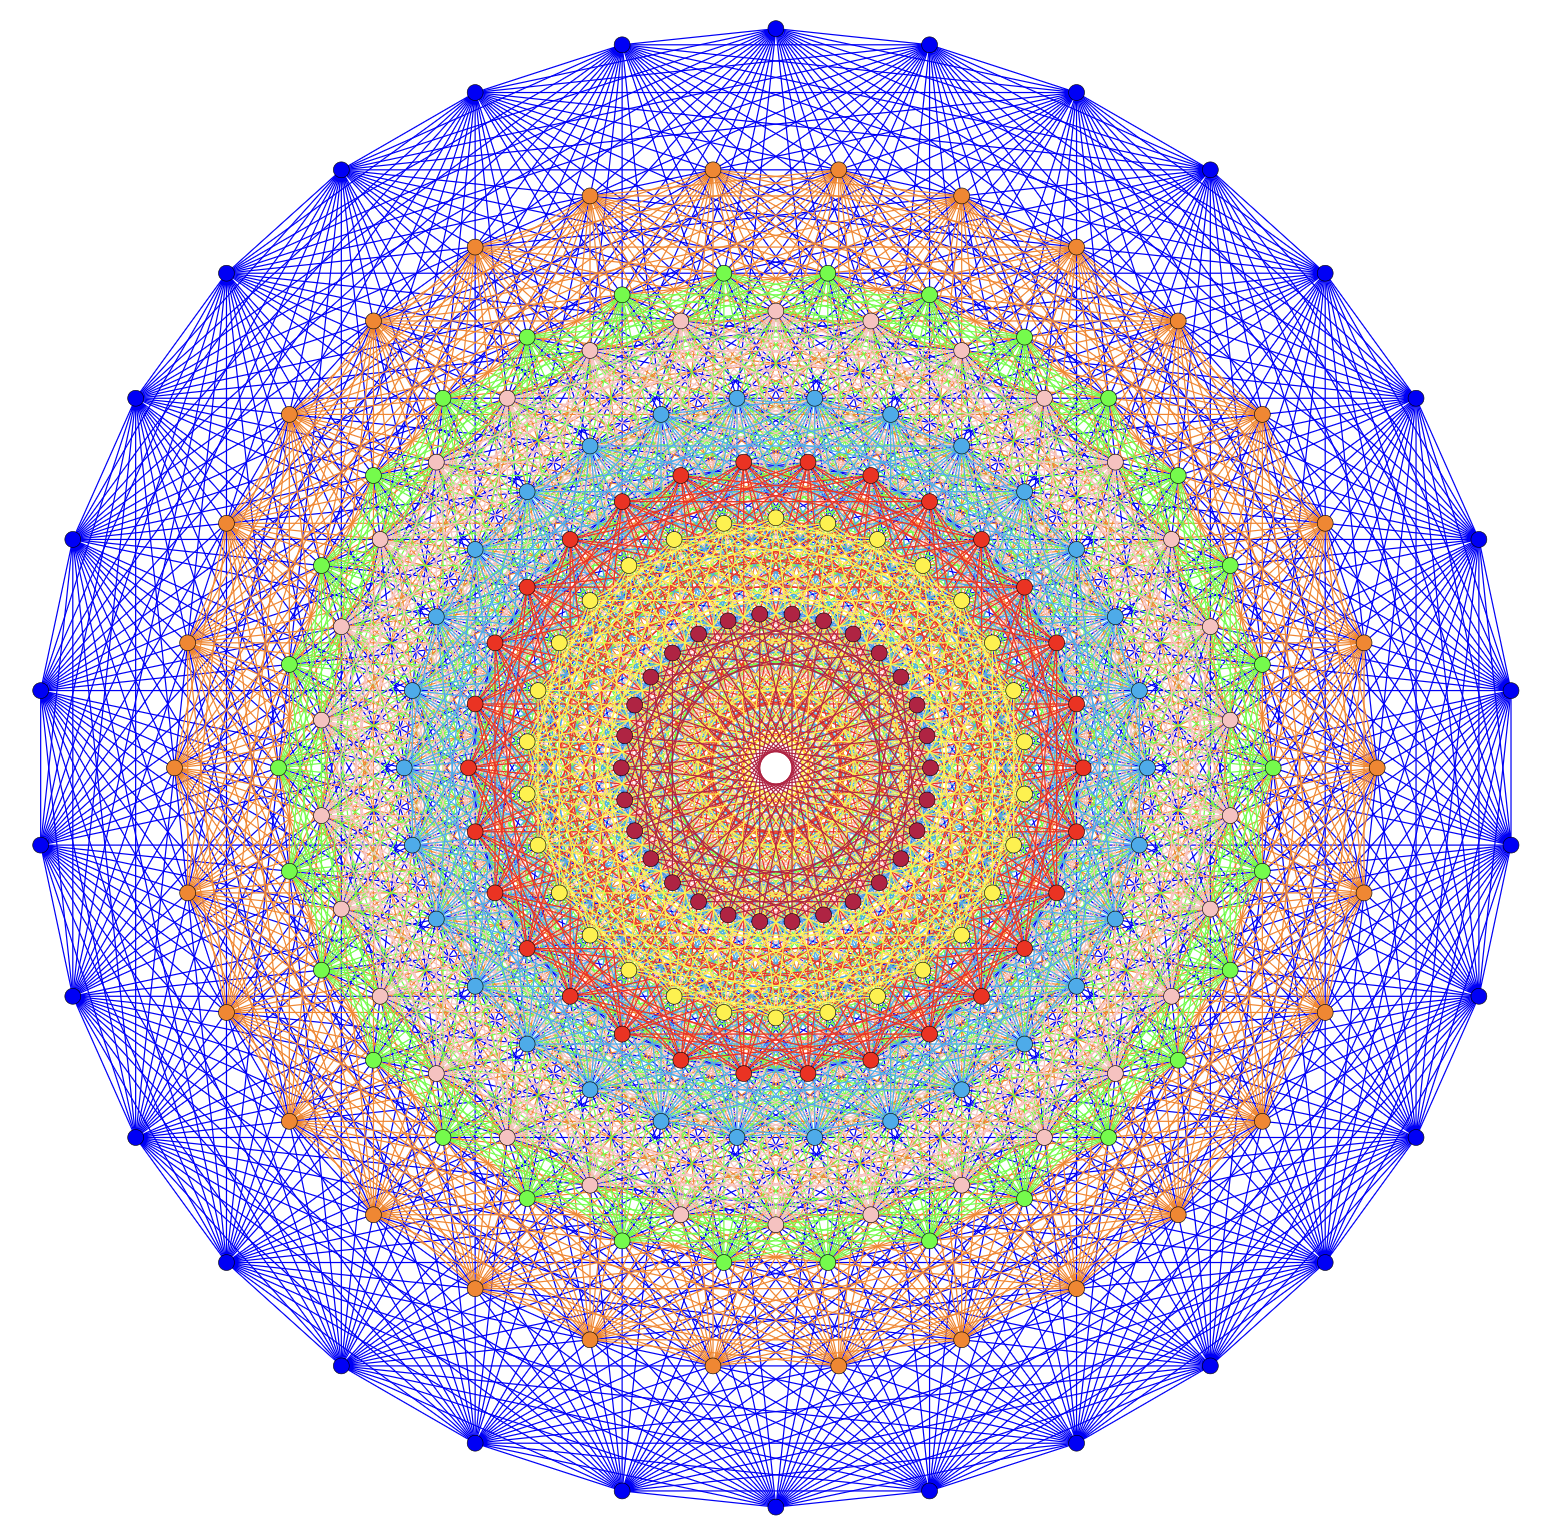
\includegraphics[width=0.98\linewidth]{Chapters/2_Dimension_8/Images/Gorbe_E8.png}
    \caption{The Coxeter projection of the $E_8$ root system. \cite{Gorbe_E8}}
    \label{Ch2:Fig:Gorbe_E8}
\end{wrapfigure}

It is quite remarkable that $E_8$ should show up when discussing sphere packings. At its core, $E_8$ is an irreducible root system. It shows up in the classification of important classes of objects like irreducible Coxeter groups, crystallographic Coxeter groups, and semi-simple Lie algebras over $\C$. $E_8$ is not a classical root system but an \textit{exceptional} root system, meaning that the geometric properties of its roots cannot be found in irreducible root systems in all dimensions.

The $E_8$ root system consists of $240$ vectors in $\R^8$ that are permuted by a certain finite subgroup of the $8$-dimensional orthogonal group. This group is sometimes referred to as the $E_8$ Coxeter group or as the Weyl group of the $E_8$ lattice. These roots can be divided into $8$ orbits, each of which corresponds to one of the `layers' of concentric circles in \Cref{Ch2:Fig:Gorbe_E8}. The dots in the figure correspond to projections of the roots onto a plane on which a specific type of element of the Coxeter group, known as a Coxeter element, acts as a rotation. This visualisation offers a convenient---and aesthetically pleasing---means of visualising this collection of $8$-dimensional vectors and appreciating some of its symmetry.

% From a motivational standpoint, this is quite important. So mention facts like distances between lattice points and things like that. Important for construction of magic function.

\sorry

\begin{boxtheorem}\label{Ch2:Thm:E8_Self_Dual}
    The dual lattice of the $E_8$ lattice is the $E_8$ lattice itself. That is, $\parenth{E_8}^* = E_8$ as free $\Z$-submodules of $\R^8$.
\end{boxtheorem}

This follows directly from the definitions of the dual lattice (\Cref{Ch2:Def:Dual_Lattice}) and the $E_8$ lattice (\sorry). This result will be useful later on, as it will give us an insight into the desired properties of the magic function.

\section{The Cohn-Elkies Linear Programming Bounds}\label{Ch2:Sec:CohnElkies}

Arguably, the result that most radically changed the sphere packing game was the linear programming bound constructed by Henry Cohn and Noam Elkies~\cite[Theorem 3.1]{CohnElkies}. The bound transforms the sphere packing problem from a geometric one to an analytic one. For all $d \in \N$, it posits the existence of a family of upper-bounds on the sphere packing constant $\Delta_d$, indexed by functions $f : \R^d \to \R$ that satisfy certain conditions.

The power of this result is that it offers a systematic approach to prove that a certain sphere packing $\Pa$ is optimal in $\R^d$. The optimality condition means that the density of $\Pa$ is equal to the sphere packing constant $\Delta_d$, which is equivalent to requiring that the density of $\Pa$ be greater than or equal to the density of any other packing in $\R^d$. The theorem proved by Cohn and Elkies tells us we can accomplish this by
\begin{enumerate}
    \item identifying a function $f : \R^d \to \R$ that satisfies the conditions of the theorem, giving an upper-bound for $\Delta_d$, and
    \item showing that the upper-bound indexed by $f$ is equal to the density of the packing $\Pa$.
\end{enumerate}
As simple as this sounds, it took close to fourteen years from the publication of Cohn and Elkies's paper for it to be used to concretely construct an optimal sphere packing. The real trick is to construct the right function $f$ to use in the process outlined above. We shall soon see the non-triviality of this task first-hand.

The original result~\cite[Theorem 3.1]{CohnElkies} is a bit different from the version that was chosen to be formalised. Firstly, the original result was stated for a very general class of functions known as \textit{admissible functions}. For our purposes, however, it suffices to look at Schwartz functions, which are not only admissible but also have useful properties that we will exploit later. We will remark, however, that at the time when Cohn and Elkies proposed their bound, it was not known that the solution to the sphere packing problem in dimensions $8$ and $24$ would only involve Schwartz functions. Furthermore, it might be possible that solutions in other dimensions would require the full generality of Cohn and Elkies's original result. Nevertheless, we will restrict our attention to Schwartz functions for the time being, not only because it is sufficient for our purposes but also because the theory of Schwartz functions has been developed quite substantially in \mathlib.

Another minor difference between the original result and the version we work with is that the original result was stated as an upper-bound on all \textit{centre densities} of sphere packings. The centre density of a sphere packing is merely a rescaling of its density by a factor of $\Volof{B_d\of{0, 1}}\inv$. Instead of encoding the information of the amount of sphere packing volume per unit volume of the ambient space, the centre density encodes the information of the number of centres of the sphere packing per unit volume of the ambient space. We sidestep these nuances by stating the result in terms of quantities we have defined.

\begin{boxtheorem}[Cohn and Elkies, 2003~{\cite[Theorem 3.1]{CohnElkies}}]\label{SP:Thm:CohnElkies} % Make sure to include the original version before this and then this adaptation
    If $f : \R^d \to \R$ is a Schwartz function satisfying the conditions
    \begin{enumerate}[label = \normalfont(CE\arabic*)]
        \item\label{SP:CE1} $f$ is not identically zero.
        \item\label{SP:CE2} For all $x \in \R^d$, if $\norm{x} \geq 1$ then $f(x) \leq 0$.
        \item\label{SP:CE3} For all $x \in \R^d$, $\hat{f}(x) \geq 0$.
    \end{enumerate}
    then we have the following bound on the sphere packing constant $\Delta_d$:
    \begin{align*}
        \Delta_d \leq \frac{f(0)}{\hat{f}(0)} \cdot \Volof{B_d\of{0, \frac{1}{2}}}
    \end{align*}
\end{boxtheorem}
\begin{proof}
    Let $f : \R^d \to \R$ be a Schwartz function satisfying the conditions~\ref{SP:CE1}-\ref{CE3}. By \Cref{Ch2:Prop:Periodic_Const_eq_Const}, it suffices to prove that
    \begin{align*}
        \Delta_d^{\text{periodic}} \leq \frac{f(0)}{\hat{f}(0)} \cdot \Volof{B_d\of{0, \frac{1}{2}}}
    \end{align*}

\end{proof}
\section{A Word on Modular Forms}
\label{Ch2:Sec:ModForms}
\chapter{A Roadmap to Constructing the Magic Function}
\label{Ch3:Chapter}
\thispagestyle{empty}

% CONSIDER MAKING THIS ENTIRE CHAPTER A SECTION OF THE NEXT CHAPTER, WITH EACH OF ITS SECTIONS BECOMING SUBSECTIONS! It will wreak havoc on our labelling system, but I don't think the contents of this chapter are enough to give it chapter status. Either that, or the sections of the previous chapter need to become chapters in their own right, which would give them more importance than they merit (seeing as they are merely background, no matter how essential).

We mentioned, in the introduction, that the scope of this project is to construct Viazovska's Magic Function in Lean and prove that it satisfies certain specific properties, such as satisfying the hypotheses of the \CELP. In this chapter, we will outline the steps we will take to achieve this goal. In particular, we will list all the conditions we need to prove that the Magic Function satisfies. Our approach will be to construct the Magic Function in terms of two intermediary functions. Proving it satisfies the necessary conditions will then be a matter of proving that these intermediary functions satisfy certain properties. We will list these properties as well.

\section{Radial Schwartz Functions}

In the statement of~\Cref{SP:Thm:CohnElkies}, we require the function in terms of which we bound the sphere packing constant in dimension $d$ to be Schwartz. However, we have yet to formally define what this means. Intuitively, a Schwartz function is a smooth function whose every derivative decays faster than any inverse power of the norm. Below, we give a more formal definition that is adapted from the definition of the \verb|structure| \verb|SchwartzMap| in \mathlib.\todo{cite}

\begin{boxdefinition}[Schwartz Function]
    Let $E$ and $F$ be normed $\R$-vector spaces. We say that $f : E \to F$ is \textbf{Schwartz} if it is infinitely continuously differentiable and for all $n, k \in \N$, there exists some $C \in \R$ such that for all $x \in E$,
    \begin{align}
        \norm{x}^k \cdot \norm{f^{(n)}(x)} \leq C
        \label{Ch3:Eq:SchwartzDecayProperty}
    \end{align}
\end{boxdefinition}

One can show that $\R$-linear combinations of Schwartz functions are Schwartz functions. Then, given any $E$ and $F$, we can define the Schwartz space $\Sch(E, F)$.

\begin{boxdefinition}[Schwartz Space]
    Let $E$ and $F$ be normed $\R$-vector spaces. We define the \textbf{Schwartz space} $\Sch(E, F)$ to be the set of all Schwartz functions from $E$ to $F$, viewed as a vector space over $\R$.
\end{boxdefinition}

At the outset, it might appear that the reason we are interested in Schwartz functions is that this is a requirement of the Poisson Summation Formula\todo{cross reference}, which is used in the proof of the \CELP\ (\Cref{SP:Thm:CohnElkies}). However, this turns out to be a sufficient condition for the Poisson Summation Formula to hold, not a necessary condition. There is a deeper reason why we are interested in Schwartz functions: the \CEC\ immediately show us that we should also consider the properties of the Fourier transform of the magic function, and Fourier transforms of Schwartz functions turn out to be Schwartz. In fact, we can say something stronger when we view the Fourier transform as an operator on the Schwartz space.

\begin{boxtheorem}\label{Ch3:Thm:FourierSchwartz_CLE}
    Let $V$ be a finite-dimensional inner-product space over $\R$ and let $E$ be a normed vector space over $\C$. The Fourier transform
    \begin{align*}
        \F : \Sch(V, E) \to \Sch(V, E) : f \mapsto \hat{f}
    \end{align*}
    is a linear isomorphism of $\Sch(V, E)$. % Leave out continuity because the discussion of the topology of the Schwartz space is not relevant.
\end{boxtheorem}

A formal proof of this result can be found in \mathlib.

It turns out that there is another condition we can impose to simplify our hunt for the magic function. The key idea is to find a function satisfying the conditions~\ref{CE1}-\ref{CE3}. Observe, for $x \in \R^d$, that \ref{CE1} does not depend on $x$, and \ref{CE2} and \ref{CE3} only depend on $\norm{x}$. This allows us to narrow our search to \textbf{radial functions}, which we define as follows.

\begin{boxdefinition}[Radial Functions]
    Let $E$ be a normed $\R$-vector space and $\alpha$ an arbitrary set. We say that $f : E \to \alpha$ is \textbf{radial} if for all $x, y \in E$, if $\norm{x} = \norm{y}$, then $f(x) = f(y)$.
\end{boxdefinition}

Radial Schwartz functions interact with the Fourier Transform in an even nicer way than ordinary Schwartz functions.

\begin{boxproposition}\label{Ch3:Prop:RadialSchwartzFourier}
    Let $f : \R^d \to \C$ be a radial Schwartz function. Then,
    \begin{align*}
        \F\of{\F\of{f}} = f
    \end{align*}
\end{boxproposition}
\begin{proof}
    Fix $x \in \R^d$. Applying \Cref{Ch2:Lemma:Fourier_Inverse_Fourier_Neg} to $\F\of{f}$ and $-x$, we have
    \begin{align*}
        \F\of{\F\of{f}}\of{x} = \F\inv\of{\F\of{f}}\of{-x} = f\of{-x} = f\of{x}
    \end{align*}
    where the fact that $\F\inv\of{\F\of{f}} = f$ follows from the fact that $f$ is Schwartz and the fact that $\fof{-x} = \fof{x}$ follows from the fact that $f$ is radial.
\end{proof}

\Cref{Ch3:Prop:RadialSchwartzFourier} indirectly provides us with a mechanism for constructing the magic function that is beautifully outlined in~\cite{CohnOnViazovskaICM}. Observe that if $f$ is a radial Schwartz function, we can write
\begin{align*}
    f = \underbrace{\frac{f - \hat{f}}{2}}_{=: f_{-}} + \underbrace{\frac{f + \hat{f}}{2}}_{=: f_{+}}
\end{align*}
The functions $f_{-}$ and $f_{+}$ have the properties that
\begin{align*}
    \F\of{f_{-}} &= \frac{1}{2} \parenth{\F\of{f} - \F\of{\hat{f}}} = \frac{1}{2} \parenth{\hat{f} - f} = -f_{-} \\
    \F\of{f_{+}} &= \frac{1}{2} \parenth{\F\of{f} + \F\of{\hat{f}}} = \frac{1}{2} \parenth{\hat{f} + f} = f_{+}
\end{align*}
where we use \Cref{Ch3:Prop:RadialSchwartzFourier} to show that $\hat{\hat{f}} = f$. In other words, $f_{-}$ and $f_{+}$ are \textbf{eigenfunctions of the Fourier transform} with eigenvalues $-1$ and $+1$ respectively. In fact, if
\begin{align*}
    f = \lambda f_1 + \mu f_2
\end{align*}
for \textit{any} two functions $f_1$ and $f_2$ such that $\hat{f_1} = -f_1$ and $\hat{f_2} = f_2$, then one can show, by computing $f_{-}$ and $f_{+}$, that $\lambda f_1 = f_{-}$ and $\mu b = f_{+}$. This allows us to break down the problem of computing the magic function into two smaller problems, namely, computing its constituent Fourier $\pm 1$-eigenfunctions.

Before discussing the other properties we seek in our magic function---or its constituent Fourier eigenfunctions---we develop some very useful machinery that allows us to show that radial functions are Schwartz. We usually treat radial functions as $\R \to \C$ functions, because all information about the input that is necessary to compute the corresponding output is captured by a (non-negative) real number: its norm. The decaying property \eqref{Ch3:Eq:SchwartzDecayProperty} of Schwartz functions is something that, at first glance, makes it a bit tricky to ignore the dimension of the domain when dealing with radial Schwartz functions. Ideally, we would want to only show that the decaying property holds for the corresponding $\R \to \C$ function. We can show this for a class of radial Schwartz functions that only depend on $\norm{x}^2$.

\begin{boxproposition}\label{Ch3:Prop:Multidimensional_Schwartz_of_Schwartz}
    Let $f : \R \to \C$ be a Schwartz function. For all $d \in \N$, the function
    \begin{align*}
        f_d : \R^d \to \C : x \mapsto \fof{\norm{x}^2}
    \end{align*}
    is Schwartz.
\end{boxproposition}

We do not prove this result here, but we do mention that there is a \sorry-free Lean proof of it in our repository.\todo{cross reference}

The point of \Cref{Ch3:Prop:Multidimensional_Schwartz_of_Schwartz} is that it gives us a criterion to show that radial functions in higher dimensions that are functions not of the norm but of the norm \textit{squared} are Schwartz, purely by considering the corresponding function that takes in a one-dimensional input. This will be instrumental in our argument.

With this, we end our discussion of radial Schwartz functions. The key takeaway is that while Schwartzness is a necessary condition for our magic function to satisfy, we can also impose the condition of radiality to simplify our construction. We will now take a closer look at Cohn and Elkies's groundbreaking result (\Cref{SP:Thm:CohnElkies}) to determine further properties for the magic function to satisfy.
\section{The \CELP, Revisited}
\label{Ch3:Sec:Cohn_Elkies_Revisited}

So far, we have examined the statement of \Cref{SP:Thm:CohnElkies} in detail: it immediately tells us that we want the magic function to be Schwartz and satisfy the conditions~\ref{CE1}-\ref{CE3}, and upon noticing that these conditions only depend on the norm and that radial functions are very well-behaved, we have narrowed our search to radial Schwartz function obeying \ref{CE1}-\ref{CE3}. It turns out that we can learn even more about the magic function when we examine the \textit{proof} of \Cref{SP:Thm:CohnElkies} when we specialise to the case where the function $f$ is optimal. Our examination of the proof of \Cref{SP:Thm:CohnElkies} is based on an insightful discussion in~\cite[p. 8]{CohnOnViazovskaICM}.

Specifically, let $f$ be a (radial) Schwartz function satisfying \ref{CE1}, \ref{CE2} and \ref{CE3}. What it means for $f$ to be optimal is that there exists a sphere packing $\Pa(X)$ in $\R^d$ such that the Cohn-Elkies bound indexed by $f$ is precisely the density of this sphere packing. This would make $\Pa(X)$ an optimal sphere packing in $\R^d$ and $f$ an optimal function.

Since it is enough to prove the upper-bound property for periodic sphere packings, we can simplify our search for the right $f$ by assuming the Cohn-Elkies bound corresponding to $f$ is the density of a \textit{periodic} packing. In other words, we can assume there exists some lattice $\Lambda \subset \R^d$ such that the set of centres $X$ is periodic with respect to $\Lambda$. This turns out to be helpful because we can then use the exact forms of the inequalities in the proof to deduce properties that $f$ must have if it is optimal, corresponding to some optimal periodic packing.

In our argument, we fix an arbitrary $\Lambda$-periodic sphere packing $\Pa(X)$ of separation $1$ and show the inequality~\eqref{Ch2:Eq:CohnElkies_Ineq_1}. In the case where $f$ is optimal, in the sense that the upper-bound is achieved, we must have that \eqref{Ch2:Eq:CohnElkies_Ineq_1} is, in fact, an \textbf{equality}. The same must be true of the equivalent inequality, \eqref{Ch2:Eq:CohnElkies_Ineq_2}. This tells us that the intermediate inequalities \eqref{Ch2:Eq:CohnElkies_Ineq_3} and \eqref{Ch2:Eq:CohnElkies_Ineq_4} must \textit{also} be equalities, because the chain of inequalities begins and ends at the same quantity. In particular, we can take a closer look at \eqref{Ch2:Eq:CohnElkies_Ineq_3}: the way we prove it is by writing
\begin{align*}
    \abs{\quotient{X}{\Lambda}}  \cdot f(0)
    = \sum_{x \in {\tiny{\quotient{X}{\Lambda}}}} \fof{x - x}
    = \sum_{x \in X} \sum_{\substack{y \in {\tiny \quotient{X}{\Lambda}} \\ y = x}}
    \geq \sum_{x \in X} \sum_{y \in {\tiny \quotient{X}{\Lambda}}} \fof{x - y}
\end{align*}
The terms we discard to prove the inequality are non-positive, as they are of the form $\fof{x - y}$ for $y \neq x$ (meaning $\norm{y - x} \geq 1$, allowing us to apply \ref{CE2}). If this inequality is an equality, then all the terms we discard must not merely be non-positive: they must, in fact, be zero. That is, we need
\begin{align}
    \fof{x - y} = 0 \text{ for all \textbf{distinct} } x \in X \text{ and } y \in \quotient{X}{\Lambda}
    \label{Ch3:Eq:OptimalFunctionVanishing_fun}
\end{align}
By definition of $\quotient{X}{\Lambda}$, \textit{every} element of $\Lambda$ is expressible as $x - y$ for some $x \in X$ and $y \in \quotient{X}{\Lambda}$, because $X$ consists of \textit{all} $\Lambda$-translates of $y$. So, all non-zero lattice points are expressible as $x - y$ for $x$ and $y$ as in \eqref{Ch3:Eq:OptimalFunctionVanishing_fun}. We can therefore conclude that \textbf{an optimal function $f$ with Cohn-Elkies bound equal to the density of a periodic sphere packing must vanish at all non-zero lattice points}.

It turns out that examining \ref{CE2} gives us an \textit{even stronger} condition on $f$. First, note that we must have $0 \leq f(0)$: the bound
\begin{align*}
    \frac{f(0)}{\hat{f}(0)} \cdot \Volof{B_d\of{0, \frac{1}{2}}}
\end{align*}
is greater than or equal to a non-negative constant, and both $\Volof{B_d\of{0, \frac{1}{2}}}$ (as a volume) and $\hat{f}(0)$ (by \ref{CE3}) are non-negative, meaning $f(0)$ cannot possibly be negative. Indeed, this is true regardless of whether $f$ is optimal. Since \ref{CE2} tells us that $f$ is non-positive at points with norm at least $1$, we can conclude that $f$ not only has zeroes but \textbf{double zeroes} at all lattice points with norm at least $1$: the behaviour of $f$, viewed as an $\R \to \R$ function of the norm $r$ of a point on $\R^d$, is such that sign-changes, if any, from non-negative to non-positive cannot occur at zeroes $\geq 1$, and thereafter, there are no more sign changes.

Putting these conclusions about single and double zeroes together with our observation about splitting radial Schwartz functions into their constituent $\pm 1$-Fourier eigenfunctions, we can conclude that we need to find \textbf{Fourier eigenfunctions with double zeroes at lattice points}. It is no accident that this is precisely the title of \cite[Section 4]{Viazovska8}.



\section{A Strategy for Constructing the Fourier Eigenfunctions}
% WHAT DO I CALL THIS SECTION????????

Before we outline the strategy used by Viazovska to construct the $\pm 1$-Fourier eigenfunctions (and subsequently, the magic function), we outline the properties we would like the magic function to have. We then examine which of these properties come from the eigenfunctions and explore ways of using this information to construct them. For the remainder of this thesis, we will fix the following notation.

\begin{boxnotation}
    Going forward, the magic function for $8$-dimensional sphere packing shall be denoted $g$, its $+1$-eigenfunction shall be denoted $a$, and its $-1$-eigenfunction shall be denoted $b$.
\end{boxnotation}

We now list the properties we would like $g$ to have.

\begin{enumerate}
    \item $g$ needs to be a Schwartz function.
    \item It suffices for $g$ to be radial.
    \item $g$ needs to satisfy the Cohn-Elkies conditions \ref{CE1}, \ref{CE2} and \ref{CE3}.
    \item $g$ needs to have single zeroes at all non-zero points in $\Lambda_8$.
    \item $g$ needs to have double zeroes at all but finitely many points in $\Lambda_8$.
    \item The \CELP\ indexed by $g$ must be equal to the density of the $E_8$ sphere packing. That is, we need
    \begin{align*}
        \frac{g(0)}{\hat{g}(0)} \cdot \Volof{B_8\of{0, \frac{1}{2}}} = \frac{\pi^4}{384}.
    \end{align*}
\end{enumerate}

Of these properties, the following would be inherited from $a$ and $b$:

\begin{enumerate}
    \item Schwartzness
    \item Radiality
    \item Having single zeroes at all non-zero points in $\Lambda_8$
    \item Having double zeroes at all but finitely many points in $\Lambda_8$
\end{enumerate}

That is, if we can construct $a$ and $b$ such that they satisfy the above properties, then $g$ will satisfy them as well. The remaining properties will have to do with the coefficients of the linear combination of $a$ and $b$ that makes up $g$.

While the properties of $g$ inform the properties we would like $a$ and $b$ to have, we construct $a$ and $b$ \textit{before} constructing $g$. That is, we are not so much constructing a magic function and splitting it into its constituent eigenfunctions as we are computing Fourier eigenfunctions and showing that a particular linear combination of them is the desired magic function. In the formalisation, too, it is necessary that the construction of $a$ and $b$ precede that of $g$. One advantage of this is that constructing $a$ and $b$ as terms of the right \verb|SchwartzMap| type means that any linear combination will yield a term of the same \verb|SchwartzMap| type, because there is a \verb|Module| instance in \mathlib\ on \verb|SchwartzMap| objects that tells us that the Schwartz space is a vector space. In similar fashion, if less directly, the other `inherited' properties will be easy to prove for the linear combination if we prove $a$ and $b$ satisfy those properties.

\begin{comment}
    ** Note: we gotta include PolyFourierCoeffBound somewhere!! **

    Maybe it's better to say ``here's how Viazovska did it'' and just outline her paper and then say ``here's what's different about the overall structure in Lean'' and outline a few things like the way we decided to structure the MagicFunction bit of the repo. Things like
    1. Wanting reusability: keeping `PolyFourierCoeffBound` separate
    2. Modularity: splitting it up from `ModularForms`
    3. Namespacing to avoid clashes (eg. a as a function and a as a SchwartzMap term)
    4. The strategy for the integrals: using real parametrisations and using straight contours instead of circular ones
\end{comment}
\chapter{Viazovska's Magic Function, Informally}
\label{Ch4:Chapter}
\thispagestyle{empty}

In this chapter, we will construct the $+1$-eigenfunction $a$, the $-1$-eigenfunction $b$, and the magic function $g$. The theory developed in \Cref{Ch3:Chapter} tells us what properties we would like all three functions to satisfy, and in \Cref{Ch3:Sec:Properties}, we summarised those properties concisely. Over the course of this chapter, we prove that they do, indeed, satisfy them.

The content is based heavily on Viazovska's original paper \cite[\S 4]{Viazovska8} and a more detailed version of her proof that she wrote originally for the project blueprint \cite[\S 7]{blueprint}. However, some details, including the very definitions of $a$ and $b$, differ slightly from the original paper. While these modifications add numerous computational inconveniences to the argument, they are necessary for the formalisation. The arguments given in this chapter are formulated to correspond either to formalised proofs or to the proof path the author has in mind for eventual formalisation, and every effort has been made to avoid assuming general results, however well-known, that have not previously been formalised. Previously formalised mathematics is assumed and applied freely, and links are provided where appropriate. The similarities and subtle differences between the approach in this report and Viazovska's original approach are discussed in greater detail in \Cref{Ch5:Sec:Gen_Overview_of_Formalisation}.

We begin by defining the functions in question. In each subsequent section of this chapter, we will prove a certain property for each of the eigenfunctions. Finally, in \Cref{Ch4:Sec:g_Properties}, we will prove that $g$ does, indeed, satisfy the properties outlined in \Cref{Ch3:Chapter}.

\section{Defining Viazovska's Fourier Eigenfunctions}

The $\pm$-eigenfunctions of $g$---and, by extension, $g$ itself---are defined in terms of modular and quasimodular forms (recall the definitions of these terms from \Cref{Ch2:Sec:ModForms}). Specifically, the $+1$-eigenfunction $a$ is defined in terms of the so-called $\phi$- and $\psi$-functions, which are in turn defined in terms of the Eisenstein series (cf. \sorry) and the discriminant form (cf. \sorry), while the $-1$-eigenfunction $b$ is defined in terms of the Jacobi Theta functions (cf. \sorry)\todo{Define in Chapter 2 and cross-ref here}.

We begin by defining the $+1$-eigenfunction $a$.

\subsection{The $+1$-Eigenfunction}

We begin by defining the $\phi$-functions.

\begin{boxdefinition}[The $\phi$-Functions]\label{Ch4:Def:phis}
    Define the functions $\phi_0, \phi_{-2}, \phi_{-4} : \Halfplane \to \C$ by
    \begin{align}
        \phi_{-4} &:= \frac{E_4^2}{\Delta}
            \label{Ch4:Eq:phi_-4_def} \\
        \phi_{-2} &:= \frac{E_4\parenth{E_2 E_4 - E_6}}{\Delta}
            \label{Ch4:Eq:phi_-2_def} \\
        \phi_{0} &:= \frac{\parenth{E_2 E_4 - E_6}^2}{\Delta}
            \label{Ch4:Eq:phi_0_def}
    \end{align}
\end{boxdefinition}

These functions admit important transformation properties that are necessary to prove that the $+1$-eigenfunction is made up of integrals of holomorphic functions. This fact will in turn allow us to apply the Cauchy-Goursat Theorem (and variants thereof) that will allow us to shift contours of integration.

\begin{boxlemma}
    For all $z \in \Halfplane$,
    \begin{align}
        \phi_0\of{z + 1}
        &= \phi_0\of{z}
        \label{Ch4:Eq:phi_0_add_one} \\
        \phi_0\of{\frac{-1}{z}}
        &= \phi_0\of{z}
        - \frac{12 i}{\pi} \cdot \frac{1}{z} \cdot \phi_{-2}\of{z}
        - \frac{36}{\pi^2} \cdot \frac{1}{z^2} \cdot \phi_{-4}\of{z}
        \label{Ch4:Eq:phi_0_neg_inv}
    \end{align}
\end{boxlemma}

The proofs of these involve transformations of $E_2$, $E_4$, $E_6$, and $\Delta$, and can be found in \cite{blueprint}. We now define the $+1$-eigenfunction $a$.

\begin{boxdefinition}[Viazovska's $+1$-Fourier Eigenfunction]\label{Ch4:Def:a}
    Define $a\rad : \R \to \C$ by
    \begin{align}
        a\rad\of{r} := I_1(r) + I_2(r) + I_3(r) + I_4(r) + I_5(r) + I_6(r)
            \label{Ch4:Eq:a_rad_def}
    \end{align}
    where, for all $r \in \R$,
    \begin{align}
        I_1(r) &:= \int_{-1}^{-1 + i} \phi_0\of{\frac{-1}{z+1}} \,
                                 \parenth{z + 1}^2 \,
                                 e^{\pi i r z} \,
                                 \diff{z}
            \label{Ch4:Eq:I_1_def} \\
        I_2(r) &:= \int_{-1 + i}^{i} \phi_0\of{\frac{-1}{z+1}} \,
                                 \parenth{z + 1}^2 \,
                                 e^{\pi i r z} \,
                                 \diff{z}
            \label{Ch4:Eq:I_2_def} \\
        I_3(r) &:= \int_{1}^{1 + i} \phi_0\of{\frac{-1}{z - 1}} \,
                                \parenth{z - 1}^2 \,
                                e^{\pi i r z} \,
                                \diff{z}
            \label{Ch4:Eq:I_3_def} \\
        I_4(r) &:= \int_{1 + i}^{i} \phi_0\of{\frac{-1}{z - 1}} \,
                                \parenth{z - 1}^2 \,
                                e^{\pi i r z} \,
                                \diff{z}
            \label{Ch4:Eq:I_4_def} \\
        I_5(r) &:= -2 \int_{0}^{i} \phi_0\of{\frac{-1}{z}} \,
                                z^2 \,
                                e^{\pi i r z} \,
                                \diff{z}
            \label{Ch4:Eq:I_5_def} \\
        I_6(r) &:= 2 \int_{i}^{i \infty} \phi_0\of{z} \,
                                e^{\pi i r z} \,
                                \diff{z}
            \label{Ch4:Eq:I_6_def}
    \end{align}
    Define the $+1$-Fourier eigenfunction $a : \R^8 \to \C$ by
    \begin{align}
        a(x) := a\rad\of{\norm{x}^2}
            \label{Ch4:Eq:a_def}
    \end{align}
\end{boxdefinition}

It is immediate from \eqref{Ch4:Eq:a_def} that $a$ is radial. All of its properties are determined by its radial part $a\rad$. There are similar definitions in Lean.

There is an important remark that must be made about the definitions in \eqref{Ch4:Eq:I_1_def}-\eqref{Ch4:Eq:I_6_def}: in the original paper \cite{Viazovska8}, the integrals $I_1$ and $I_2$ are combined, as are $I_3$ and $I_4$, and expressed in the following manner:
\begin{align*}
    I_1(r) + I_2(r) &= \int_{-1}^{i} \phi_0\of{\frac{-1}{z+1}} \, \parenth{z + 1}^2 \, e^{\pi i r z} \, \diff{z} \\
    I_3(r) + I_4(r) &= \int_{1}^{i} \phi_0\of{\frac{-1}{z - 1}} \, \parenth{z - 1}^2 \, e^{\pi i r z} \, \diff{z}
\end{align*}
with the contours not specified. The most `classical' choice would be quarter-circular contours, though the same results can be achieved working with straight and rectangular contours.

\begin{figure}[ht]
    \centering
    % First subfigure: quarter-circular contour
    \begin{subfigure}{0.3\textwidth}
        \centering
        \begin{tikzpicture}[scale=1]
            % Axes
            \draw[->] (-2.2,0) -- (2.2,0) node[right] {Re};
            \draw[->] (0,-2.2) -- (0,2.2) node[above] {Im};

            % Quarter-circle from -1 to 1 (semi-circle in upper half)
            \draw[thick, domain=180:0] plot ({cos(\x)}, {sin(\x)});
            % Arrow in middle (at 90 degrees)
            \draw[->, thick] (0,-1) arc (-90:-80:1);
        \end{tikzpicture}
        \caption{Quarter-circular contour}
    \end{subfigure}
    \hfill
    % Second subfigure: straight line
    \begin{subfigure}{0.3\textwidth}
        \centering
        \begin{tikzpicture}[scale=1]
            % Axes
            \draw[->] (-2.2,0) -- (2.2,0) node[right] {Re};
            \draw[->] (0,-2.2) -- (0,2.2) node[above] {Im};

            % Straight line from -1 to 1
            \draw[thick, ->] (-1,0) -- (0,0);
            \draw[thick] (0,0) -- (1,0);
        \end{tikzpicture}
        \caption{Straight line from $-1$ to $1$}
    \end{subfigure}
    \hfill
    % Third subfigure: rectangular contour
    \begin{subfigure}{0.3\textwidth}
        \centering
        \begin{tikzpicture}[scale=1]
            % Axes
            \draw[->] (-2.2,0) -- (2.2,0) node[right] {Re};
            \draw[->] (0,-2.2) -- (0,2.2) node[above] {Im};

            % Rectangular contour
            \draw[thick] (-1,0) -- (-1,1);
            \draw[thick] (-1,1) -- (0,1);

            % Arrows indicating direction
            \draw[->, thick] (-1,0.5) -- (-1,0.51); % upward
            \draw[->, thick] (-0.5,1) -- (-0.49,1); % rightward
        \end{tikzpicture}
        \caption{Rectangular contour}
    \end{subfigure}
    \caption{Different contour choices for the integrals that make up $a$}
    \label{Ch4:fig:a_contours}
\end{figure}

The reason the choice of contours does not matter is that in the integrands of $I_1, \ldots, I_5$, we multiply terms of the form $\phi_0\of{\frac{-1}{z}}$ by $z^2$. If we apply \eqref{Ch4:Eq:phi_0_neg_inv} and multiply through, it is clear that we are removing any singularities introduced by $\frac{1}{z^2}$ and $\frac{1}{z}$ factors. We can then use the fact that $\Delta\of{z} \neq 0$ for all $z \in \Halfplane$ to conclude that the integrands are holomorphic up to these removable singularities.

% Insert a visual here for I_1, and say I_2 is analogous

We are now ready to define the $-1$-eigenfunction $b$.

\subsection{The $-1$-Eigenfunction}

Recall the definitions of the $H$-functions defined in \sorry\ to be the fourth powers of the thetanullwerte. We begin by defining the $\psi$-functions in terms of these $H$-functions.\todo{check these with original paper}

\begin{boxdefinition}[The $\psi$-Fucntions]\label{Ch4:Def:psis}
    Define the functions $\psi_I, \psi_S, \psi_T : \Halfplane \to \C$ by
    \begin{align}
        \psi_I &:= \frac{H_4^3\parenth{2 H_4^2 + 5 H_4 H_2 + 5 H_2^2}}{2 \Delta}
            \label{Ch4:Eq:psi_I_def} \\
        \psi_S &:= \frac{- H_2^3 \parenth{2 H_2^3 + 5 H_2 H_4 + 5 H_4^2}}{2 \Delta}
            \label{Ch4:Eq:psi_S_def} \\
        \psi_T &:= \psi_I - \psi_S
            \label{Ch4:Eq:psi_T_def}
    \end{align}
    
\end{boxdefinition}
\section{Establishing the Schwartzness Property}

We know that the Schwartz space is a $\C$-vector space, making it closed under addition. To show that $a$ and $b$ are Schwartz functions, we show that their constituent integrals $I_1, \ldots, I_6$ and $J_1, \ldots, J_6$ are Schwartz. We need to show both smoothness and rapid decay. Smoothness is fairly straightforward. Rapid decay, on the other hand, requires an additional ingredient.

It turns out that we can establish a general result that yields an upper-bound for functions of the form $\frac{f}{\Delta}$, where $\Delta$ is the discriminant form and there is a polynomial growth condition on the Fourier coefficients of $f$. We take advantage of the fact that the $\phi$- and $\psi$-functions can be expressed in this form (cf. \Cref{Ch4:Def:phis} and \Cref{Ch4:Prop:psi_as_div_disc}). The condition on their Fourier coefficients comes from the theory of modular forms.

We begin with the statement and proof of the general result \cite[Lemma 7.4]{blueprint}.\todo{UPDATE LEMMA NUMBER BEFORE SUBMITTING}

\begin{boxtheorem}\label{SP:PolyFourierCoeffBound}
    Let $f : \C \to \C$ be holomorphic. Denote by $c_f(n)$ its $n$th Fourier coefficient of $f$ with $c_f\of{n_0} \neq 0$, so that
    \begin{align*}
        f(z) = \sum_{n=n_0}^{\infty} c_f(n) \, e^{i \pi n z}
    \end{align*}
    If $c_f(n)$ has polynomial growth in $n$---that is, if there exists $k \in \N$ such that $c_f(n) = \BigO{n^k}$---then there exists a constant $C_f > 0$ such that for all $z \in \Halfplane$ with $\Im\of{z} \geq \frac{1}{2}$,
    \begin{align*}
        \abs{\frac{f(z)}{\Delta(z)}} \leq C_f \, e^{-\pi \parenth{n_0 - 2} \Im(z)}
    \end{align*}
\end{boxtheorem}
\begin{proof}
    
\end{proof}

\subsection{The $+1$-Eigenfunction}

\subsection{The $-1$-Eigenfunction}
\section{Establishing the Eigenfunction Property}

% Prove that the 2 eigenfunctions are, indeed, Fourier eigenfunctions!

In this section, we show that the $\pm$-Eigenfunctions are, indeed, $\pm$-Eigenfunctions of the Fourier transform.

In the previous section, we did not really work 

\subsection{The $+1$-Eigenfunction}

\subsection{The $-1$-Eigenfunction}
\section{Establishing the Double Zeroes Property}

\subsection{The $+1$-Eigenfunction}

\subsection{The $-1$-Eigenfunction}
\section{Another Representation of the Eigenfunctions}
\label{Ch4:Sec:Analytic_Cont}

At this stage, it is worth consolidating the results proven thus far. In \Cref{Ch3:Sec:Properties}, we mentioned numerous \textit{necessary} conditions for eigenfunctions to satisfy. The fact that it is immensely difficult to find functions satisfying such conditions, juxtaposed with the fact that we have done precisely that, is an indication that we are on the right track. However, it is still not clear how to compute $g$ as a linear combination of $a$ and $b$ and show it satisfies \ref{CE1}-\ref{CE3}, we need information about the behaviour of $a\rad$ and $b\rad$ on specific points in $\Ico{0, \infty}$.

It will turn out that \ref{CE2} is a consequence of the alternate representations of $a$ and $b$ constructed in \Cref{Ch4:Sec:Double_Zeroes}. $d$ and $c$, however, are only defined on $\parenth{2, \infty}$, so they do not provide us with information on what happens closer to $0$, which we need for \ref{CE3}. Viazovska's solution was to analytically continue $d$ and $c$ to all of $\Ico{0, \infty}$. This will help us prove not only \ref{CE3} but also \ref{CE1}. Moreover, it will help us show that the Cohn-Elkies bound we get in the end does indeed give us the density of the $\Lambda_8$.

\subsection{The $+1$-Eigenfunction}

We begin by defining the following integral.

\begin{boxdefinition}
    Define $\tilde{d} : \Ico{0, \infty} \to \R$ by
    \begin{align*}
        \tilde{d}(r) :=&
        4i \sinsq{\frac{\pi r}{2}} \Bigg(
        -\frac{36}{\pi^3\parenth{r - 2}} + \frac{8640}{\pi^3 r^2} - \frac{18144}{\pi^3 r} \\
        &+\int_{0}^{\infty} \parenth{t^2 \phi_0\of{\frac{i}{t}} - \frac{36}{\pi^2}e^{2\pi t} + \frac{8640}{\pi} - \frac{18144}{\pi^2}} e^{-\pi r t} \, \diff{t}\Bigg)
    \end{align*}
\end{boxdefinition}

Observe that for $r > 2$
\begin{align*}
    \int_{0}^{\infty} \parenth{\frac{36}{\pi^2}e^{2\pi t} - \frac{8640}{\pi} + \frac{18144}{\pi^2}} e^{-\pi r t} \, \diff{t}
    = \frac{36}{\pi^3\parenth{r - 2}} - \frac{8640}{\pi^3 r^2} + \frac{18144}{\pi^3 r}
\end{align*}
Thus, for all $r > 2$, $\tilde{d} = d$. So, $\tilde{d}$ is a continuation of $d$  from $\parenth{2, \infty}$ to $\Ico{0, \infty}$. However, it is not immediately clear that $\tilde{d}$ is analytic.

Viazovska proceeds by computing the Fourier expansion of $\phi_0\of{i/t}$ and showing that
\begin{align*}
    t^2 \, \phi_0\of{\frac{i}{t}} =
    \frac{36}{\pi^2}e^{2\pi t} - \frac{8640}{\pi} + \frac{18144}{\pi^2} + \BigO{t^2 \, e^{-2 \pi t}}
\end{align*}
as $t \to \infty$ \cite[(39)]{Viazovska8}. One can then conclude that the integral in $\tilde{d}$ converges absolutely for all $r \geq 0$. It is then clear that $\tilde{d}$ is analytic on $\Ico{0, \infty}$. Since $a\rad$ is smooth, hence analytic,\todo{state this in Lean} on $\Ico{0, \infty}$ as well, by the identity principle for analytic functions, which has \href{https://github.com/leanprover-community/mathlib4/blob/6c6e0180f0d3dc9f47f85532f48d268d8656789a/Mathlib/Analysis/Analytic/Uniqueness.lean#L217-L226}{previously been formalised}, we can conclude that $a\rad = \tilde{d}$ on $\Ico{0, \infty}$.

Finally, we note that
\begin{align*}
    a\of{0} = a\rad\of{0} = \tilde{d}\of{0} = \frac{-i 8640}{\pi}
\end{align*}

\subsection{The $-1$-Eigenfunction}

We proceed analogously.

\begin{boxdefinition}
    Define $\tilde{c} : \Ico{0, \infty} \to \R$ by
    \begin{align*}
        \tilde{d}(r) :=&
        4i \sinsq{\frac{\pi r}{2}} \Bigg(
        \frac{144}{\pi r} + \frac{1}{\pi\parenth{r - 2}} + \\
        &+\int_{0}^{\infty} \parenth{\psi_I\of{it} - 144 - e^{2 \pi t}} e^{-\pi r t} \, \diff{t}\Bigg)
    \end{align*}
\end{boxdefinition}

Observe that for $r > 2$
\begin{align*}
    \int_{0}^{\infty} \parenth{144 + e^{2 \pi t}} e^{-\pi r t} \, \diff{t}
    = \frac{144}{\pi r} + \frac{1}{\pi\parenth{r - 2}}
\end{align*}
Thus, for all $r > 2$, $\tilde{c} = c$. So, $\tilde{c}$ is clearly a continuation of $c$ from $\parenth{2, \infty}$ to $\Ico{0, \infty}$. However, it is not immediately clear that $\tilde{c}$ is analytic.

Again, Viazovska proceeds by computing the Fourier expansion of $\psi_I\of{it}$ and showing that
\begin{align*}
    \phi_I\of{it} =
    144 + e^{2\pit} + \BigO{e^{- \pi t}}
\end{align*}
as $t \to \infty$ \cite[(39)]{Viazovska8}. One can then conclude that the integral in $\tilde{c}$ converges absolutely for all $r \geq 0$. It is then clear that $\tilde{c}$ is analytic on $\Ico{0, \infty}$. We conclude just as we did for $a$.


\section{The Magic of $g$}
\label{Ch4:Sec:g_Properties}

% Cohn-Elkies conditions: 
\chapter{Viazovska's Magic Function, Formally}
\label{Ch5:Chapter}
\thispagestyle{empty}
% I really don't like this chapter name because idt it reflects the essence of the chapter, which is "the key aspects of the formalisation/challenges faced and overcome". But that's not a good title either. Gotta find something in the middle!

In this chapter, we discuss aspects of the formalisation that we alluded to, but did not discuss in detail, in \Cref{Ch4:Chapter}.

Throughout \Cref{Ch4:Chapter}, particularly in \Cref{Ch4:Sec:Defs,Ch4:Sec:Schwartzness,Ch4:Sec:Double_Zeroes}, we provided incredibly detailed arguments. The purpose of doing this was to ensure a correspondence between the informal text in this document and the formal proof or proof path written or envisioned by the author. This approach was also intended to pre-empt challenges that would be faced when ultimately formalising Viazovska's proof.

We note that while the formalisation is still actively in progress, over the course of this M4R, the author has made significant progress towards formalising the contents of \Cref{Ch4:Chapter}. These steps are highlighted across this chapter. In \Cref{Ch5:Sec:Gen_Overview_of_Formalisation}, we give a broad overview of the author's contributions and account for the minor but deliberate and carefully considered differences between Viazovska's original proof in \cite{Viazovska8} and the author's exposition of it in \Cref{Ch4:Chapter}.  In \Cref{Ch5:Sec:Meta}, we briefly discuss an innovative approach conceived by Macbeth and the author to simplify computations in $\C$, which has since been implemented with significant contributions by Xie. In \Cref{Ch5:Sec:Cauchy-Goursat}, we discuss the nuances that make the \CGT, an integral part of Viazovska's proof, a challenging theorem to formalise, and outline how some, but not all, of these challenges have been overcome by the author over the course of this M4R.

\section{Project Design}

\begin{comment}
Things like
1. Repo structure/organisation
2. What the blueprint and dependency graph are and how to interpret them
3. Plan to go public
Make this very very very short. No need to ramble about stuff that doesn't warrant it. But need to make it clear that this is being done very professionally.
\end{comment}
\section{A Metaprogramming Approach}
\label{Ch5:Sec:Meta}

\begin{comment}
Begin by saying a few words about what metaprogramming is. Then go into subsections. Idea:
1. Establish difficulty of doing computations in \C. Give examples, yes, but also stress that existing automation was unable to unpack the structural nuances of the way \C is defined. Also maybe talk about the whole "is I a numeral" debate, but I think this might be a rabbit-hole...
2. Talk about the algorithm behind norm_numI. Talk about the original version we worked on with Heather and Edison at/after metaprogramming and at Xena.
3. Say something about what Heather's latest modifications look like. Maybe also talk about how the approach can be generalised to quaternion algebras or splitting fields (what's similar and what's different between norm_numI and these things), but don't talk about the maths of either of these. Stress that this is still under development, and that this opens the door to a world of metaprogramming possibilities.
\end{comment}

The formalisation of the solution to the sphere packing problem brought to light a longstanding difficulty faced by the Lean community: a lack of automation for performing computations in $\C$. After a discussion with Heather Macbeth, who is experienced in creating automation for Lean, the author, with Macbeth's guidance and Xie's assistance, embarked on the development of a normalisation-simplification automation procedure for performing computations in the complex numbers.

% I will condense the stuff below in the shorter (for-submission) version of this thesis. I'll leave it as is over here though... maybe this will come in handy someday...

Lean, like other interactive theorem provers, primarily interacts with its users through \textbf{tactics}. Fundamentally, the proof of a theorem in Lean is given by a \textbf{proof term}, which can be thought of as a concise expression that captures the information of how the hypotheses or inputs of the theorem are transformed into its conclusion by giving exactly the conclusion into which these inputs are transformed. A tactic is a command that, when invoked by a Lean user, performs a step in the construction of the proof term for a theorem.

The most basic tactics can be thought of as being `syntax sugar' rather than invocations of computation or reasoning algorithms. Consider the following code.
% MORE LATEX ERRORS! GAHHHHHHHH
% \begin{lstlisting}[caption=A tactic-mode proof of the associativity of $\land$, label=Ch5:Listing:And_assoc_tactic]
% example (P Q R : Prop) : P ∧ (Q ∧ R) ↔ (P ∧ Q) ∧ R := by
%   constructor
%   · intro h
%     constructor
%     · constructor
%       · exact h.1
%       · exact h.2.1
%     · exact h.2.2
%   · intro h
%     constructor
%     · exact h.1.1
%     · constructor
%       · exact h.1.2
%       · exact h.2
% \end{lstlisting}

This proof demonstrates how the \lstinline|constructor|, \lstinline|intro| and \lstinline|exact| tactics work. These tactics give the Lean compiler the following instructions:
\begin{itemize}
    \item \lstinline|constructor|: ``Prove the goal by proving the two statements it consists of." It works on conjunctions and biconditionals, that is, if the goal is of the form \lstinline|A ∧ B|, then \lstinline|constructor| replaces it with two goals, namely, \lstinline|A| and \lstinline|B|, and if the goal is of the form \lstinline|A ↔ B|, then \lstinline|constructor| replaces it with two goals, namely, \lstinline|A → B| and \lstinline|B → A|.
    
    \item \lstinline|intro|: ``Prove the goal by introducing the assumption term and proving the conclusion term." It works on implications and universal quantifications, that is, if the goal is of the form \lstinline|A → B|, then \lstinline|intro h| introduces an assumption \lstinline|h| of \lstinline|A| and replaces the goal with \lstinline|B|, and if the goal is of the form \lstinline|∀ (x : A), B|, then \lstinline|intro a| introduces term \lstinline|a| of type \lstinline|A| and replaces the goal with \lstinline|B|.

    \item \lstinline|exact|: ``Prove the goal with the following." It works on any goal where the proof of that goal is already known, that is, if the goal is \verb|B| and some proof \lstinline|h| of \lstinline|B| is already known, then \lstinline|exact h| proves the goal with \lstinline|h|.
\end{itemize}

In addition, the terms \lstinline|h.1|, \lstinline|h.2.1|, etc are shorthand for ``the first constituent of \lstinline|h|'', ``the first constituent of (the second constituent of \lstinline|h|)'', etc, where by ``first constituent'' and ``second constituent'', we mean the terms respectively to the left and right of the $\land$ symbol.

What the tactics used in \Cref{Ch5:Listing:And_assoc_tactic} are actually doing is constructing the following \textbf{term-mode proof} of the same result.

\begin{lstlisting}[caption=A term-mode proof of the associativity of $\land$, label=Ch5:Listing:And_assoc_term]
example (P Q R : Prop) : P ∧ (Q ∧ R) ↔ (P ∧ Q) ∧ R :=
  ⟨fun h ↦ ⟨⟨h.1, h.2.1⟩, h.2.2⟩,
   fun h ↦ ⟨h.1.1, ⟨h.1.2, h.2⟩⟩⟩
\end{lstlisting}

% Try and end the discussion here. The point we were trying to make is that tactics generate proof terms. I think that point has been made! The remainder of this section can maybe be a discussion in an appendix. We can say something like "here's some fun facts about theorem proving in Lean" and include this and maybe even some other fun stuff from the book

This proof is significantly shorter than the tactic-mode proof see in \Cref{Ch5:Listing:And_assoc_tactic}. While the code is arguably less readable than the tactic-mode proof, it is not too difficult to dissect:
\begin{itemize}
    \item The \lstinline|constructor| occurrences in \Cref{Ch5:Listing:And_assoc_tactic} correspond to the \textit{anonymous constructors} \lstinline|⟨,⟩| in \Cref{Ch5:Listing:And_assoc_term}.

    \item The \lstinline|intro h| occurrences in \Cref{Ch5:Listing:And_assoc_tactic} correspond to the function definitions \lstinline|fun h ↦| in \Cref{Ch5:Listing:And_assoc_term}.

    \item The \lstinline|exact| occurrences in \Cref{Ch5:Listing:And_assoc_tactic} correspond to the terms inside the anonymous constructors in \Cref{Ch5:Listing:And_assoc_term}.
\end{itemize}

In particular, the proof in \Cref{Ch5:Listing:And_assoc_term} consists solely of functions and constructors. No tactics occur anywhere in the argument (note the absence of the \lstinline|by| keyword, which marks the beginning of a tactic-mode proof).

It turns out that \Cref{Ch5:Listing:And_assoc_term} still contains some syntax sugar. It is possible to use helper lemmas like \verb|Iff.intro| and \verb|And.intro| to avoid using the anonymous constructors, but a proof term completely devoid of the constructor syntax would look like the following.

% Why am I getting LaTeX errors here????????
% \begin{lstlisting}[caption=A proof term for the associativity of $\land$, label=Ch5:Listing:And_assoc_proof_term, escapeinside=``]
% example (P Q R : Prop) : P ∧ (Q ∧ R) ↔ (P ∧ Q) ∧ R := {
%   mp := fun a ↦ {
%     left := {
%       left := And.casesOn a fun left right ↦ And.casesOn right fun _ _ ↦ left
%       right := And.casesOn a fun _ right ↦ And.casesOn right fun left _ ↦ left
%     }
%     right := And.casesOn a fun _ right ↦ And.casesOn right fun _ right ↦ right
%   }
%   mpr := fun a ↦ {
%     left := And.casesOn a fun left _right ↦ And.casesOn left fun left _ ↦ left `\newpage`
%     right := {
%       left := And.casesOn a fun left _ ↦ And.casesOn left fun _ right ↦ right
%       right := And.casesOn a fun left right ↦ And.casesOn left fun _ _ ↦ right
%     }
%   }
% }
% \end{lstlisting}

Proof terms, as we can see from \Cref{Ch5:Listing:And_assoc_proof_term}, are often long and do not clearly communicate the mathematical ideas they represent. Tactics overcome this by constructing proof terms without revealing them to the user. Indeed, there are tactics that serve as more than just syntax sugar: for example, results in intuitionistic propositional logic (such as the associativity of $\land$) can be proved by the tactic \lstinline|itauto|. That is, the following code compiles.


\begin{lstlisting}[caption=A one-line tactic proof for the associativity of $\land$, label=Ch5:Listing:And_assoc_itauto]
example (P Q R : Prop) : P ∧ (Q ∧ R) ↔ (P ∧ Q) ∧ R := by itauto
\end{lstlisting}

Other tactics like \lstinline|tauto| and \lstinline|simp| also work. The proof term generated by such a tactic can be viewed by typing \lstinline|show_term|.\footnote{For the curious reader, \Cref{Ch5:Listing:And_assoc_proof_term} was generated by repeatedly typing \lstinline|show_term by tauto| inside each field.} For a more detailed explanation of how proof terms and tactics work, see \cite[particularly Chapters 3 and 5]{ThmPfInLean}.

\textbf{Metaprogramming} is the science of writing tactics in Lean. While syntax-sugar tactics are incredibly useful (compare the readability of \Cref{Ch5:Listing:And_assoc_tactic,Ch5:Listing:And_assoc_term,Ch5:Listing:And_assoc_proof_term}), automation tactics often go an even longer way in keeping the focus of nontrivial mathematical proofs on precisely their nontrivial aspects. Given how computationally involved the construction of Viazovska's Magic Function is (as seen in \Cref{Ch4:Chapter}), the author, after a discussions with Macbeth, realised that the most efficient approach to formalising some of the computational aspects of Viazovska's argument was to write a tactic. The first version of this tactic, developed as a collaboration between Macbeth, Xie and the author, with inputs from Mehta, was called \lstinline|norm_numI|.

In the forthcoming subsections, we explore the motivation and technique used to develop \lstinline|norm_numI|, and briefly discuss how the tactic maybe further developed and the scope of its applicability expanded.

\subsection{Complex Computations are Complex}

Computations in general are quite challenging to perform in interactive theorem provers. This is because such languages are designed for \textit{proof} rather than \textit{computation}. Indeed, tactics that simplify goals do not do so merely by simplifying expressions: they construct proofs that the simplified expression is, indeed, equal to the original expression. Existing tactics like \lstinline|norm_num|, \lstinline|simp| and \lstinline|field_simp| do not always do this successfully when the expressions in question are in $\C$. \lstinline|simp| and \lstinline|field_simp| are very general tactics that work in a wide variety of settings. They both work by constructing a special set of equality or biconditional lemmas by sifting through the library and performing repeated rewrite operations to transform the goal into a simpler form. \lstinline|field_simp| is specifically designed to simplify expressions in fields, and can handle operations like clearing denominators. However, it does not have access to the particularities of the field in question (such as the fact that $i^2 = -1$ in $\C$). The tactic that we will be most interested in, specifically because it is designed to handle simplifications of \textit{numerals} in \textit{specific} settings, is \lstinline|norm_num|.

\lstinline|norm_num| is a tactic that handles expressions involving numerals. It works best in $\N$, $\Z$ and $\Q$. For example, it handles the following.
% \begin{lstlisting}[caption={\lstinline|norm_num| simplifying expressions in $\N$, $\Z$ and $\Q$}]
% example : (1 : ℕ) + 2 + 3 + 4 = 10 := by norm_num
% example : (-2 : ℚ) * (3 + 8/9) = -70/9 := by norm_num
% example : (-9 : ℤ) + 5 * (6 - 20) = -79 := by norm_num
% \end{lstlisting}
It is worth mentioning, however, that \lstinline|norm_num| often has difficulties in $\R$. This is due to the immense technical detail baked into the very definition of $\R$ in Lean, which allows for the existence of transcendental numbers. In the following example, none of \lstinline|norm_num|, \lstinline|field_simp|, \lstinline|ring| and \lstinline|simp| can prove the result in one line, because they are unable to treat $\pi$ as more than a symbol. Indeed, the entire proof rests on a \mathlib\ result, \lstinline|Real.pi_gt_three|.

\begin{lstlisting}[caption=An expression in $\R$ not handled immediately by simplification tactics, label=Ch5:Listing:pi_sub_one_norm_num_fail]
example : (π - 1) / (π - 1) = 1 := by
  have h₁ : (1 : ℝ) < 3 := by norm_num
  have h₂ : 1 ≠ π := ne_of_lt <| h₁.trans pi_gt_three
  have h₃ : π - 1 ≠ 0 := sub_ne_zero_of_ne h₂.symm
  field_simp [h₃]
\end{lstlisting}

Observe, however, that \lstinline|norm_num| \textit{is} able to prove the inequality $1 < 3$ despite it being an expression in $\R$. The reason is that \lstinline|norm_num| can navigate the canonical inclusions from $\N$, $\Z$ and $\Q$ into $\R$, meaning that it can simplify expressions in $\R$ that come from expressions it can simplify in $\N$, $\Z$ or $\Q$.\footnote{We say \lstinline|norm_num| can handle coercions.} It cannot, however, show that $1 < \pi$, because it does not treat $\pi$ \textit{as a numeral}. In $\C$, \lstinline|norm_num| faces this challenge not only with real transcendental numbers like $\pi$ but also with the imaginary constant $i$. Consider the following example.\footnote{Note that in Lean, the imaginary constant is denoted by an uppercase \lstinline|I| instead of a lowercase $i$. We will adhere to standard mathematical conventions and use a lowercase $i$ when referring to the imaginary constant in informal contexts.}

\begin{lstlisting}[caption={A nontrivial computation in $\C$, done formally}, label=Ch5:Listing:long_tactic_pf_example_complex]
example : (1 + I) * (1 + I * I * I) = 2 := by
  simp only [I_mul_I, neg_mul, one_mul, mul_add, mul_one, mul_neg, add_mul, neg_add_rev, neg_neg]
  ring
\end{lstlisting}

Again, \lstinline|simp|, \lstinline|field_simp|, \lstinline|ring| and \lstinline|norm_num| all fail, because $i$, like $\pi$ in \Cref{Ch5:Listing:pi_sub_one_norm_num_fail}, is not handled as a numeral. Observe, however, that $\parenth{1 + i}\parenth{1 + i \cdot i \cdot i}$ lies in $\Z[i]$. This means that if it is expressed as $a + bi$, with $a$ and $b$ both being (not necessarily simplified) real expressions, then in fact, $a$ and $b$ are both images of expressions in $\Z$. This means that \lstinline|norm_num| would be able to individually handle both $a$ and $b$, resulting in a simplified expression of the form $a' + b'i$, with $a'$ and $b'$ being simplified. This suggests that the key to writing a tactic that can simplify expressions like those in \Cref{Ch5:Listing:long_tactic_pf_example_complex} is to find a way to separate them into their real and imaginary parts, which in turn involves navigating the fact that $i^2 = -1$.

\subsection{Parsing and Normalisation}

The core idea behind \lstinline|norm_num| is that it simplifies expressions by computing normal forms. In its most basic form, \lstinline|norm_num| attempts to prove equalities of by putting the left and right hand sides in unique normal forms that can simply be inspected to check if the two sides are equal. For example, in the natural numbers, simple arithmetic facts are true by \textit{reflexivity}, that is, they are proved by the tactic \lstinline|rfl|, which proves definitional equality. Hence, the right normal form for numerical expressions in $\N$ is to just compute them and express them as a single natural number (ie, as the right number of applications of the successor function to $0$). Then, by inspection, two expressions are equal if and only if their normal forms---that is, their simplifications into single natural numbers---are equal. Inequalities work similarly.

While the working of \lstinline|norm_num| may appear trivial in $\N$, its versatility becomes clearer in \textit{semirings}. Recall that a semiring is an algebraic structure that is a commutative, additive monoid and a multiplicative monoid, with the quintessential example being $\N$. If $A$ is any semiring, there is a natural semiring homomorphism $\uparrow : \N \to A$ given by
\begin{align*}
    \uparrow\!0 &:= 0 \\
    \uparrow\!1 &:= 1 \\
    \uparrow\!2 &:= 1 + 1 \\
    &\ \ \ \vdots
\end{align*}
A \textbf{numeral} in $A$ is then any element of the image of $\uparrow$, and \lstinline|norm_num| puts expressions involving numerals in normal forms by recognising them as numerals, computing the normal form of their pre-images in $\uparrow$, and pushing the image back through $\uparrow$. The nontriviality of \lstinline|norm_num| for numerical expressions in $A$ is then not how it computes normal forms in $\N$ but how it navigates $\uparrow$. For more on how \lstinline|norm_num| works in semirings, follow the tutorial in \cite[\texttt{Metaprogramming/NormNum}]{HeatherMetaprogramming}. We will not discuss it in any more detail here, but will instead discuss the working of \lstinline|norm_numI|---specifically, what the desired normal form is and how it is computed.

Since $\R$ is a subfield of $\C$, the constraints that the standard \lstinline|norm_num| faces in $\R$ are also constraints it can reasonably be expected to face in $\C$. The goal of \lstinline|norm_numI| is not to overcome \textit{these} constraints, but to overcome the \textit{additional} constraints that come from not treating $i$ as a numeral. The target normal form for an expression in $\C$ is therefore given by separating it into its real and imaginary parts, both of which are real expressions, and normalising them as much as possible.

The key to \lstinline|norm_numI| is the \href{https://github.com/thefundamentaltheor3m/Sphere-Packing-Lean/blob/05f51ee8f61972da1b0a5ee360c4c57c1b599cca/SpherePacking/Tactic/NormNumI.lean#L72}{\lstinline|parse| function}. It separates an expression $z \in \C$ into its real and imaginary parts by performing a recursive pattern-match. For example, if the outermost operation is addition---ie, if $z = z_1 + z_2$---then it calls itself on both $z_j$, obtaining real and imaginary parts $a_j, b_j \in \R$ and proofs that $z_j = a_j + b_ji$, and returns the expression $\parenth{a_1 + a_2} + \parenth{b_1 + b_2}i$ as well as a proof that $z = \parenth{a_1 + a_2} + \parenth{b_1 + b_2}i$, which it obtains via a helper lemma \href{https://github.com/thefundamentaltheor3m/Sphere-Packing-Lean/blob/05f51ee8f61972da1b0a5ee360c4c57c1b599cca/SpherePacking/Tactic/NormNumI.lean#L20}{\lstinline|split_add|}. It performs similar recursive actions if $z$ is of the form $z_1 \cdot z_2$, $z_1\inv$, $z_1 / z_2$, $-z_1$, $z_1 - z_2$, $\overline{z_1}$, $z_1^n$ for some $n \in \N$, $i$, or a decimal/natural number. The recursion is guaranteed to terminate, because an expression that is fed into the function cannot contain infinitely many characters.

\begin{boxexample}\label{Ch5:Eg:Parse}
    The expression $z = \parenth{1 + i}\parenth{1 + i \cdot i \cdot i}$ (cf. \Cref{Ch5:Listing:long_tactic_pf_example_complex}) would be parsed in the following manner.
    \begin{enumerate}[noitemsep]
        \item To parse $z$, write $z = z_1 \cdot z_2$, where $z_1 = 1 + i$ and $z_2 = 1 + i \cdot i \cdot i$.
        \item To parse $z_1$, write $z_1 = z_{11} + z_{12}$ where $z_{11} = 1$ and $z_{12} = i$.
        \item $z_{11}$ is parsed as $1 + 0i$.
        \item $z_{12}$ is parsed as $0 + 1i$.
        \item By \lstinline|split_add|, $z_1 = z_{11} + z_{12}$ is parsed as
              \begin{align*}
                  \parenth{1 + 0} + \parenth{0 + 1}i
              \end{align*}
        \item To parse $z_2$, write $z_2 = z_{21} + z_{22}$, where $z_{21} = 1$ and $z_{22} = i \cdot i \cdot i$.
        \item $z_{21}$ is parsed as $1 + 0i$.
        \item To parse $z_{22}$, write $z_{22} = z_{221} \cdot z_{222}$, where $z_{221} = i \cdot i$ and $z_{222} = i$.
        \item To parse $z_{221}$, write $z_{221} = z_{2211} \cdot z_{2212}$, where $z_{2211} = i$ and $z_{2212} = i$.
        \item $z_{2211}$ is parsed as $0 + 1i$.
        \item $z_{2212}$ is parsed as $0 + 1i$.
        \item By \lstinline|split_mul|, $z_{221} = z_{2211} \cdot z_{2212}$ is parsed as
              \begin{align*}
                  \parenth{0 \cdot 0 - 1 \cdot 1} + \parenth{0 \cdot 1 + 0 \cdot 1}i
              \end{align*}
        \item $z_{222}$ is parsed as $0 + 1i$.
        \item By \lstinline|split_mul|, $z_{22} = z_{221} \cdot z_{222}$ is parsed as
              \begin{align*}
                  \parenth{
                    \parenth{0 \cdot 0 - 1 \cdot 1}
                        \cdot
                    0
                    -
                    \parenth{0 \cdot 1 + 1 \cdot 0}
                        \cdot
                    1
                  } + \parenth{
                    \parenth{0 \cdot 0 - 1 \cdot 1}
                        \cdot
                    1
                    +
                    0
                        \cdot
                    \parenth{0 \cdot 1 + 1 \cdot 0}
                  }i
              \end{align*}
        \item By \lstinline|split_add|, $z_2 = z_{21} + z_{22}$ is parsed as
              \begin{align*}
                  &\parenth{1 + \parenth{
                    \parenth{0 \cdot 0 - 1 \cdot 1}
                        \cdot
                    0
                    -
                    \parenth{0 \cdot 1 + 1 \cdot 0}
                        \cdot
                    1
                  }} \\
                  + &\parenth{0 + \parenth{
                    \parenth{0 \cdot 0 - 1 \cdot 1}
                        \cdot
                    1
                    +
                    0
                        \cdot
                    \parenth{0 \cdot 1 + 1 \cdot 0}
                  }}i
              \end{align*}
        \item By \lstinline|split_mul|, $z = z_1 + z_2$ is parsed as
              \hspace{-2em}
              \begin{align*}
                  &\Big(
                    \parenth{1 + 0}
                        \cdot
                    \parenth{1 + \parenth{
                        \parenth{0 \cdot 0 - 1 \cdot 1}
                            \cdot
                        0
                        -
                        \parenth{0 \cdot 1 + 1 \cdot 0}
                            \cdot
                        1
                    }} \\
                    & -
                    \parenth{0 + 1}
                        \cdot
                    \parenth{0 + \parenth{
                        \parenth{0 \cdot 0 - 1 \cdot 1}
                            \cdot
                        1
                        +
                        0
                            \cdot
                        \parenth{0 \cdot 1 + 1 \cdot 0}
                    }}
                  \Big) \\
                  + &\Big(
                    \parenth{1 + 0}
                        \cdot
                    \parenth{0 + \parenth{
                        \parenth{0 \cdot 0 - 1 \cdot 1}
                            \cdot
                        1
                        +
                        0
                            \cdot
                        \parenth{0 \cdot 1 + 1 \cdot 0}
                    }} \\
                    & +
                    \parenth{1 + \parenth{
                        \parenth{0 \cdot 0 - 1 \cdot 1}
                            \cdot
                        0
                        -
                        \parenth{0 \cdot 1 + 1 \cdot 0}
                            \cdot
                        1
                    }}
                        \cdot
                    \parenth{0 + 1}
                  \Big)i
              \end{align*}
    \end{enumerate}
\end{boxexample}

\begin{wrapfigure}{r}{0.4\linewidth}
    \centering
    \includegraphics[width=0.95\linewidth]{Chapters/5_Lean/Images/norm_numI_parse_output.png}
    \caption{The Lean output of the steps shown in \Cref{Ch5:Eg:Parse}.}
    \label{Ch5:Fig:Parse_Example}
\end{wrapfigure}

Note that in Lean, the result of parsing does not appear as an expression of the form $a + bi$, but rather, as a \lstinline|structure| with fields \lstinline|re| and \lstinline|im| for the real and imaginary parts. However, the underlying idea is no different from what we have described.

Clearly, despite being mathematically valid, the result of parsing can be long and uninformative, making it an unsuitable choice of normal form for our purposes. However, by separating complex expressions into their real and imaginary parts, \lstinline|parse| perfectly sets up a very simple normalisation procedure that will put our expression in an appropriate normal form. Since we know of such a procedure for real expressions---namely, \lstinline|norm_num|---and since \lstinline|parse| expresses any complex expression as a combination of two real expressions, the normalisation procedure simply makes calls to \lstinline|norm_num| to express each of them in a \textit{real} normal form. The result is a complex number in a normal form $a + bi$ (or, in Lean notation, \lstinline|{re := a, im := b}|) with $a$ and $b$ both simplified to the greatest extent possible (as expressions in $\R$) by applying \lstinline|norm_num|.

Note that \lstinline|norm_numI| is currently implemented as a \lstinline|conv| tactic rather than a full tactic, meaning that it is only capable of modifying expressions (and providing a proof that the modification is valid). It is not currently capable of proving goals, which are necessarily logical statements, such as equalities. This means that it needs to be used as follows.

% Why is there an error in the following listing?
% Uncomment before submitting. Keep commented till then so easier to keep track of errors.
% \begin{lstlisting}[caption={Using \lstinline|norm_numI| as a \lstinline|conv| tactic}, label=Ch5:Listing:norm_numI_as_conv]
% example : (1 + I) * (1 + I * I * I) = 2 := by
%   conv_lhs => norm_numI
%   conv_rhs => norm_numI
% \end{lstlisting}

Unpacking the code,
\begin{itemize}
    \item \lstinline|conv_lhs => norm_numI| applies the parsing-normalisation procedure outlined above to convert the expression \lstinline|(1 + I) * (1 + I * I * I)| on the left-hand side to \lstinline|{re := 2, im := 0}|.
    \item \lstinline|conv_rhs => norm_numI| applies the parsing-normalisation procedure outlined above to convert the expression \lstinline|2| on the right-hand side to \lstinline|{re := 2, im := 0}|.
\end{itemize} 
Since the two sides are then exactly the same, the goal is proved. Note that both lines are necessary: $2$ on its own has not been separated into real and imaginary parts. The imaginary part needs to be explicitly shown to be $0$, which the \lstinline|parse| function does.

After Macbeth, Xie and the author's initial success with this \lstinline|conv| tactic, Macbeth proceeded to create an \textit{extension} of the existing \lstinline|norm_num| tactic that uses the parsing technique outlined above to handle complex expressions. This tactic is still being developed, but is being tested on active code from the project with immensely promising results.

\subsection{Scope for Further Development}

The benefits of having such a tactic cannot be overstated. There are numerous instances across the project where the collaborators have had to repeatedly prove computational facts in $\C$, such as $1 + i \neq 0$, or clear complex denominators to separate expressions into their real and imaginary parts. It is precisely this that motivated the development of \lstinline|norm_numI|, and indeed, \lstinline|norm_numI| is proving to be a viable solution.

% Give an explicit example here from the repo

The applicability of \lstinline|norm_numI|---or, at the very least, of the underlying idea, that the right normal form for expressions in $\C$ is to separate them into real and imaginary parts and express those in a normal form---extends well beyond expressions in $\C$. A key motivation for Xie, one of the co-creators of \lstinline|norm_numI| and an ardent algebraist, was to create a similar tactic that would normalise and simplify expressions in quaternion algebras. A discussion at a London Learning Lean event hosted at the London Institute of Mathematical Sciences in March 2025 sparked speculation among well-regarded members of the Lean Community that similar ideas might be applicable in other field extensions (with $\C$ regarded as $\quotient{\R[X]}{\parenth{X^2 + 1}}$ and $i$ as the image of $X$ via the quotient map). The idea would be that the separation into components corresponds to taking advantage of some linear independence criterion, with algebraic dependences not handled by the simplification step being captured by the helper lemmas in the normalisation step.

There are numerous technical difficulties with implementing such a tactic that can work in other contexts, chief amongst them the fact that there would need to be a single modification to the tactic capable of handling very differently behaved algebraic structures (for instance, it would need to work the same way in quadratic, cubic, quartic and higher degree field extensions). It would hence need to have some awareness of the behaviours of each field in which it is applied, which is technically challenging. Nevertheless, the development of \lstinline|norm_numI| and the subsequent \lstinline|norm_num| modification marks a significant, and long overdue, step in the right direction, so that fewer nontrivial proofs are needed to prove trivial facts.
\section{The Cauchy-Goursat Theorem}
\label{Ch5:Sec:Cauchy-Goursat}

\begin{comment}
Maybe begin with an anecdote - no sooner had we entered Hales's office in Pittsburgh than he asked about how we plan to deform integration contours.

Have 3 subsections.
1. Informal maths
2. Discussion of existing formalisation of closed rectangular case, with emphasis on why we don't have it for other cases (cite Hales's formalisation of the Jordan Curve Theorem in HOL-Light, maybe try and explain why we don't have something similar in Lean)
3. Discussion of our approach to the indefinite case (informally and formally)
Also maybe find better words than closed/open? Because these words are NOT used here in a topological sense, but rather in a very visual sense ("are the two endpoints of the curve the same point or are they not? Does the curve even have two endpoints or does it just have one and then go off to i\infty in the other?")
\end{comment}

There are some areas of mathematics that are notoriously difficult to formalise. Algebra, for example, tends to be easier to formalise than analysis. Within analysis, it tends to be particularly difficult to formalise geometric ideas. The Jordan Curve Theorem, for example, tends to be a particularly difficult theorem to formalise. It was not until 2007 that this theorem, proposed in the late 19th Century, was formalised by Tom Hales \cite{JordanCurve} in HOL Light, and to this day, no formalisation exists in Lean. The author had the privilege of meeting Hales in Pittsburgh, USA, in March 2025 to discuss the formalisation of $8$-dimensional sphere packing in Lean, and the very first question Hales asked was what the strategy was to overcome the challenges of not having a Lean formalisation of the Jordan Curve Theorem. It turns out that there is a workaround, which we explore in this section.

Before we discuss the workaround, we briefly discuss the statement of the \JCT\ and its relevance to this project. The \JCT\ essentially states that a simple closed curve $C \subset \R^2$, given as the image of a continuous injection from $\mathbb{S}^1$, divides $\R^2 \setminus C$ into a bounded region, known as the \textit{interior} of $C$, and an unbounded region, known as the \textit{exterior} of $C$. The relevance of the \JCT\ is that in Viazovska's construction---specifically, in the proof that $a$ and $b$ satisfy the double zero property---it becomes necessary to deform contours. While the contours in question are not closed, the proof that the deformation is possible (under a vanishing condition) follows from limiting applications of the Cauchy-Goursat Theorem, which states that integral of $\C \to \C$ function around a closed contour is zero if the function is holomorphic in the interior. The point is that the \JCT\ is necessary to define the interior, and without some version of the \JCT, it becomes challenging to state the all-important holomorphicity condition of the \CGT.

While it may not appear, at first, that there \textit{is} a workaround, it turns out that weaker versions of the \CGT, where the interior is more easily defined, are sufficient for our purposes. We outline the bounded and unbounded versions of these below.

% Are these section names too informal? :)

\subsection{Rectangles}

\subsection{Circles and Rectangles}
\chapter{Conclusion}
\label{Ch6:Chapter}
\thispagestyle{empty}

Over the course of this thesis, we have explored a revolutionary approach to a classical problem that has since led to deeper insights into the mysteries of the $E_8$ lattice, its $24$-dimensional counterpart, the Leech lattice, and the broader theory of radial Schwartz functions. Previously unexplored links to the theory of modular forms are revealing deep symmetries that lead to fascinating results, such as Cohn, Kumar, Miller, Radchenko and Viazovska's universal optimality and Fourier interpolation formulas \cite{UniversalOptimality} that reconstruct radial Schwartz functions $f$ from the values and radial derivatives of $f$ and $\hat{f}$, generalising Viazovska's approach to solving the sphere packing problem in $\R^8$. 

\section{Viazovska's Monumental Breakthrough}

It is with good reason that Cohn writes,
\begin{quote}
    Overall, this proof feels like a miracle.Everything falls beautifully into place, with Viazovska’s constructions having just enough flexibility to complete the proof in a unique way. \ldots Viazovska is a master of special functions, whose work would surely have excited Jacobi and Ramanujan
\end{quote}
\cite[p.21]{CohnOnViazovskaICM}. Viazovska's ingenuity stems from the manner in which she overcame the difficulties in controlling funtions and their Fourier transforms simultaneously: realising that the magic function would need to be an integral transform and that the function being transformed would need to admit numerous change of variable properties, she tapped into the theory of modular forms to find precisely such a function.

Over the course of this thesis, we have explored the specifics of how she does this. When we first encountered modular forms in \Cref{Ch2:Sec:ModForms}, it was already remarkable to observe that these 
\section{The Road to Formalising Sphere Packing}
\section{A Glance Ahead}

Despite still being fairly far from complete, this formalisation effort has all the makings of a paradigm-shifter, both for the formalisation community and the mathematics community at large. Already, the fact that \mathlib\ is at a stage where it is possible to envision a formalisation of such recent and revolutionary work as Viazovska's says volumes about the progress in formalisation over the last decade. Moreover, it is a testament to the power of open-source collaboration: every day, strides are being made by countless contributors worldwide that enhance the capabilities of Lean and the vastness of \mathlib, making for a more efficient and enjoyable formalisation experience. It is to harness the power of this community and to mobilise enthusiasts and experts to contribute to this project that the collaborators, represented by Viazovska herself, have decided to make the repository public on 13 June, 2025, at Cambridge.

Beyond the specifics of this project, the goals as well as the accomplishments thus far have a wide range of applications. For example, the author's bridge between dimensions involving Schwartz-like functions, seen in \Cref{Ch5:Subsec:Schwartz_Bridge}, and the fact that the Schwartz-like behaves nicely with linear combinations, as used in \Cref{Ch4:Sec:Schwartzness} to prove that $a\rad$ and $b\rad$ are Schwartz-like, suggests that there is a deeper theory waiting to be explored, an exciting prospect so soon after Viazovska added a revolutionary new perspective to the theory of Schwartz functions. On the formal front, the development of \lstinline|norm_numI| at a time when there is much discussion on improving automation in a variety of algebraic settings could lead to further improvements being made to existing tactics, potentially leading to the development of polymorphic automation, where normalisations and simplifications understand and depend on the setting. Furthermore, just as this project catalysed the development of \lstinline|norm_numI|, so too may it catalyse formalisations of results like the \CGT\ and potentially even the \JCT, so that future formalisers can sidesteps the vexation faced by the author when dealing with contour integrals. Finally, the systematic approach taken by the author to bound integrals formally demonstrates that a certain degree of systematisation is possible, and the author's growing understanding of metaprogramming has led to the birth---though not much more---of ideas that would make formal integral calculations more user-friendly.

The road ahead may be uncertain, but it is safe to say it is filled with potential. In conclusion, the end of this M4R is only the beginning.

% \appendix
% \input{Appendices/appendix1.tex}

%%%%%%%%%%%%%%%%%%%%%%%%%%%%%%%%%%%%%
\bibliography{./References/bibliography.bib}
% \thispagestyle{empty}
%%%%%%%%%%%%%%%%%%%%%%%%%%%%%%%%%%%%%

\end{document}